\documentclass{article}
\usepackage{amsmath}
\usepackage{graphicx}
\usepackage{subfigure}
\usepackage{fancyhdr}
\pagestyle{fancy}
\fancypagestyle{firststyle}
{
   \fancyhf{}
   \fancyfoot[l]{\footnotesize LLNL-TR-643858. This work was performed under the auspices of the U.S. Department of Energy (DOE) by Lawrence Livermore National Laboratory under Contract DE-AC52-07NA27344}
}
\title{A study of fluid-structure interaction on overlapping grids with a focus on flexible beams}
\author{Alex Main}
% LLNL-TR-643858 (released 2013/09/15 
\begin{document}
\maketitle
% \begin{figure}[h!t]
%         \centering
%         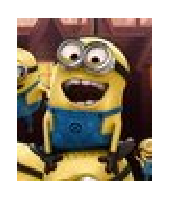
\includegraphics[width=0.2\textwidth]{minion} 
% \end{figure}
\section{Introduction}
\thispagestyle{firststyle}
Fluid-structure interaction problems appear in many areas of science and engineering.  
Adequately understanding these problems is crucial to the study of such disciplines as aeroelastic flutter, wind turbine performance, implosions and explosions, and hemodynamics, to name a few.
One technique to explore these problems is the use of numerical simulations.  
Although methods for the accurate and efficient numerical simulation of many problems involving only flexible structures or those involving only fluids have existed for a long time, the simulation of coupled problems, in which a flexible structure (or structures) interact with fluids remains challenging.
The source of the difficulty with these problems is the construction of schemes for the coupling between the fluid and the solid that are both accurate and stable.  
There are two general approaches to designing a coupling procedure.  
In the first, the so-called monolithic approach, a single solver is implemented that handles both the fluid equations and the solid equations in a single framework.  
In this scheme, the solver handles the fluid and solid equations simultaneously, resulting in a \emph{strong} coupling between the two.
The second approach, named the partitioned approach, handles the fluid and structure domains separately.  
Whereas in the monolithic scheme there is a single solver for both the fluid and the structure, in the partitioned scheme there are separate solvers for the fluid and the structure.
This separation heavily restricts the communication and coordination that can occur between the two solvers. 
Typically the only communication done in these schemes is through the application of boundary conditions (where the fluid applies a boundary condition on the fluid, and the solid one (or more) on the fluid).
This makes the implementation of partitioned schemes easy, especially because they can take advantage of existing algorithms and software developed for the simulation of fluid flow or computational mechanics.
However, they have a weakness -- accuracy and stability are much harder to achieve.
Stability is a particular problem for these schemes, as they are prone to the so-called added-mass effect.

This document examines these issues for partitioned schemes on overlapping grids.  
The use of overlapping grids is profitable for fluid-structure interaction because it obviates the need for complex and time consuming remeshing stages necessary in purely body conforming methods, while at the same time avoiding the complicated boundary conditions (and accompanying instabilities or inaccuracies) that are required for embedded (or immersed) boundary methods.
With an overlapping grid, there are two or more meshes used for the fluid domain.  
The first is a body fitted mesh around the deformable structure (or meshes around deformable structures, if there is more than one structure).  
It is on this mesh that the kinematic conditions are applied, and where the load transfer is done.
As the structure deforms, this mesh is deformed so that it remains body conforming.
The second mesh, the background mesh, remains fixed.  
It is on this mesh that inflow, outflow, and wall (for non-moving walls) boundary conditions are applied.
The meshes communicate information in their \emph{overlap} areas.  
In these areas, the fluid flow solver handles the interpolation of the necessary variables between the meshes as necessary.
Having two meshes also provides a natural framework to handle structures that significantly deform our undergo large motion.
Because the first mesh, which surrounds the structure, is structured, it is easy to regenerate when the body moves and deforms.
After this remeshing, the only further meshing operation required is the recomputation of the overlap areas between the mesh around the structure and the background mesh(es).
Because all of these meshes are structured grids, this operation is fast.  
These properties therefore make overlapping grids aptly suited for the computation of highly nonlinear fluid-structure interaction problems.

In section 2, we describe a model incompressible flow problem interacting with a flexible beam, building on the work of \cite{Causin2004}, in order to elucidate the issues involved with the coupling procedure.
We utilize the theory developed in section 2 in section 3, in which we propose and validate an implementation of our beam model and coupling procedure in the overlapping grid package consisting of Overture and CG.  
Section 4 describes an extension to this model to handle beams that are not fixed in one place (that is, free to fly around like a sheet of paper).
Section 5 describes a more sophisticated nonlinear beam model, and its coupling with the CG set of flow solvers.
Finally, section 6 describes future extensions that can be done to this work.
All of the sections contain a plethora of verification and validation data demonstrating the good performance obtained with the family of beam models implemented in the CG framework.

\section{Preliminaries}
In this first section, we describe a model problem for incompressible flow interacting with a flexible Euler-Bernoulli beam, in which the flow is inviscid, incompressible, and in which the nonlinear convective acceleration term is negligible.
We analyze its properties,  prove some stability results, and examine the added-mass effect on this problem.
This section relies heavily on the work of P. Causin \emph{et al}. \cite{Causin2004}. \\
Consider the problem: \\
{\it Find $w = w(x,t)$, ${\bf u}={\bf u}(x,y,t)$, $p = p(x,y,t)$ such that }
\begin{equation} \left\{ \begin{array}{ll}
 EI\frac{\partial^4 w}{\partial x^4}+\rho_s b h \frac{\partial ^2 w}{\partial t^2}-p(x,H)b=0 & \text{ in } (0,T) \times \Omega_S \\[0.3em]
\rho_f \frac{\partial {\bf u}}{\partial t} + \nabla p = 0 &  \text{ in } (0,T) \times \Omega_F \\
\nabla \cdot {\bf u} = 0 &  \text{ in } (0,T) \times \Omega_F \\
{\bf u} \cdot {\bf n} = \frac{\partial w}{\partial t}(x,t) & \text{ on } \Sigma \\
w(\partial \Omega_S) = w''(\partial \Omega_S) = 0
\end{array} \right. \label{eq:eq2400} \end{equation}
where $\Sigma = \overline{\Omega}_F \cap \Omega_S$.
We will take $\Omega_F$ to be a rectangle: $\Omega_F = (0,L) \times (0,H)$.
For simplicity let us assume periodic boundary conditions on the left and right of the domain.
First we use the divergence condition to introduce the pressure Poisson equation:
\begin{equation} \left\{ \begin{array}{ll}
\nabla^2 p = 0  &  \text{ in } (0,T) \times \Omega_F \\
\frac{\partial p}{\partial n} = 0 &\text{ on } \Gamma \\
\frac{\partial p}{\partial n} = -\rho_f\frac{\partial^2 w}{\partial t^2} &\text{ on } \Sigma \\
p(0,y) = p(L,y) \\
\frac{\partial p}{\partial n}(0,y) =  -\frac{\partial p}{\partial n}(L,y)
\end{array} \right. \label{eq:eq2500} \end{equation}
Now consider the function space
\begin{equation} W=\{ w \in H_0^2(\Omega_S), w''(0)=w''(H)=0 \} \label{eq:2600} \end{equation}
\begin{equation} Q=\{q \in H^1(\Omega_S), \int_{\Omega_F} q \ d \Omega_F = 0, \ q(0,y) = q(L,y) \} \label{eq:2700} \end{equation}
The weak form of the problem consisting of (\ref{eq:eq2500}) and the first equation of (\ref{eq:eq2400}) is \\
{\it Find $(w,p) \in [(0,T); W]\times [(0,T); Q]$ s.t. $\forall (v,q) \in W \times Q$},
\begin{equation} \left\{ \begin{array}{ll}
a_F(p,q) &= -\rho_f\int_\Sigma \frac{\partial ^2 w}{\partial t^2}q \ d\Sigma \\
\rho_s b h(\ddot{w},v) + EIa_S(w,v) &= \int_{\Sigma }p(x,t)v \ dx
\end{array} \right. \label{eq:eq2800} \end{equation}
where
\begin{equation} a_F(p,q) = \int_{\Omega_F} \nabla p \cdot \nabla q \ d\Omega_F \label{eq:eq2900} \end{equation}
\begin{equation} a_S(w,v) = \int_{\Omega_F} \frac{\partial^2 w}{\partial x^2} \frac{\partial^2 v}{\partial x^2}\ d\Omega_S  \label{eq:eq3000} \end{equation}
By the Lax-Milgram theorem there exists an operator $Z$ for the first equation
\[ Z : (-\rho_f \ddot{w}) \mapsto p \] 
that is given a $\ddot w$ there exists a unique $p$ satisfying the pressure Poisson equation.
Now let $\Pi_{\Sigma} : W \mapsto H^1(\Omega_S)$ be the restriction operator of $p$ to the boundary of $\Omega_F$. 
Then the operator 
\[ \Pi_{\Sigma} Z \]
is positive, and self-adjoint with respect to the $L^2(\Omega_S)$ inner product. 
Positivity follows from 
\[ (\Pi_{\Sigma} Z \ddot{w}, \ddot{w}) = -\int_{\Sigma} \ddot{w} p \ d\Sigma = \frac{1}{\rho_f}a_F(p,p) \geq 0 \]
and likewise self-adjointness:
\[  \frac{1}{\rho_f}a_F(Zw, Zv) = -\int_{\Sigma} w \Pi_{\Sigma} Z v \ d\Sigma = -\int_{\Sigma} v \Pi_{\Sigma} Z w \ d\Sigma = (\Pi_{\Sigma} Z w, v) =  (\Pi_{\Sigma} Z v, w) \] 
Using the operator $\Pi_{\Sigma} Z$ we can rewrite the second equation of (\ref{eq:eq2800}) as 
\begin{equation} ((\rho_sbh\mathcal{I}+\rho_f \Pi_{\Sigma}Z)\ddot{w}, v) + EI a_S(w,v) = 0 \label{eq:eq3100} \end{equation}
Now, let the operator $T$ be defined such that
\begin{equation}  (l,\xi) = a_S(Tl, \xi)  \label{eq:eq3200} \end{equation}
Now $T$ is self adjoint with respect to the inner product defined by $a_S(\cdot, \cdot)$, because
\[ a_S(Tv,w) = (v,w) = a_S(v,Tw) \]
Applying (\ref{eq:eq3200}) to transform equation (\ref{eq:eq3100}), 
\begin{equation} a_S(T(\rho_sbh\mathcal{I}+\rho_f \Pi_{\Sigma}Z)\ddot{w}, v) + EI a_S(w,v) = 0 \label{eq:eq3300} \end{equation}
Then because $T$ and $\rho_sbh\mathcal{I}+\rho_f \Pi_{\Sigma}Z$ are self-adjoint operators, so is
\begin{equation} A = T(\rho_sbh\mathcal{I}+\rho_f \Pi_{\Sigma}Z)\ddot{w} \label{eq:eq3400}  \end{equation}
so that $A$ has an orthonormal set of eigenvectors and eigenvalues, $(\phi_i, \mu_i)$.  
Then we can decompose and $w \in W$ as 
\begin{equation} w = \sum_{i=1}^{\infty} a_i \phi_i \label{eq:eq3500}  \end{equation}
Using this decomposition in (\ref{eq:eq3300}), we get
\begin{equation} \ddot{a}_i \mu_i + EI a_i = 0 \label{eq:eq3600}  \end{equation}
This forms a sequence of linear, constant coefficient ODE's, whose solutions therefore always exist for all $t$.  
Thus the solution of the original coupled problem exists.
Now consider the implicit time stepping scheme
\begin{equation}
\begin{aligned}
\dot{w}^{n+1} &= \dot{w}^n+\Delta t\ddot{w}^{n+1} \\
w^{n+1} &= w^n+\Delta t\dot{w}^{n+1}  
\label{eq:eq3700}
\end{aligned}
\end{equation}
Using the expansion of $w$ into the eigenvectors of A, we have
\begin{equation}
\begin{aligned}
a_i^{n+1} &= a_i^n+\Delta t \dot{a}_i^{n+1} \\
\dot{a}_i^{n+1} &= \dot{a}_i^n - \frac{EI}{\mu_i} \Delta t a_i^{n+1}
\label{eq:eq3800}
\end{aligned}
\end{equation}
This is a system with an amplification matrix
\[ \begin{bmatrix}
1 & -\Delta t \\
\frac{EI}{\mu_i}\Delta t & 1 
\end{bmatrix}^{-1}
\]
whose eigenvalues are defined by the equation
\[ 1-\lambda^{-1} = \pm i \Delta t^2 \frac{EI}{\mu_i} \]
Clearly the eigenvalues satisfy
\[ | \lambda | \leq 1 \]
and so the time stepping scheme is unconditionally stable.
In practice, however, we do not have the eigenvalues and eigenvectors.  
Rather, we must solve equations (\ref{eq:eq3100}), (\ref{eq:eq3800}) using an iterative method:
\begin{equation}
\begin{aligned}
0 &= ((\rho_sbh\mathcal{I}+\rho_f \Pi_{\Sigma}Z)\ddot{w}^{n+1}, v) + EI a_S(w^{n+1},v) \ \forall v \in W \\
\dot{w}^{n+1} &= \dot{w}^n+\Delta t\ddot{w}^{n+1} \\
w^{n+1} &= w^n+\Delta t\dot{w}^{n+1} 
\end{aligned}
\label{eq:eq3850}
\end{equation}
One classic method is a fixed point method, in which at each iteration the system 
\begin{equation} \begin{aligned}
&(\rho_sbh\tilde{\ddot{w}}^{n+1}, v) + \Delta t^2 EI a_S(\tilde{\ddot{w}}^{n+1},v)= \\
&(-\rho_f \Pi_{\Sigma}Z\ddot{w}^{(n+1,k)},v)- EI a_S(w^n,v)-EI\Delta t a_S(\dot{w}^n,v)
\end{aligned}
\label{eq:eq3860}
\end{equation}
is solved, and then the estimate for the solution $\ddot{w}^{n+1}$ is updated as (where $\omega$ is a relaxation parameter)
\[ \ddot{w}^{(n+1,k+1)} = \omega\tilde{\ddot{w}}^{n+1} + (1-\omega)\ddot{w}^{(n+1,k)} \]
It is desirable to analyze this iterative procedure to determine under what conditions it converges. 
Our analysis will differ slightly from that of \cite{Causin2004}, in that we consider a more complicated structural model.
To handle these complications, let us introduce 
\[ M: V \to V' \]
as the operator s.t.
\[ M\tilde{\ddot{w}}^{n+1} = (\rho_sbh\tilde{\ddot{w}}^{n+1}, \cdot) + \Delta t^2 EI a_S(\tilde{\ddot{w}}^{n+1},\cdot) \]
and
\[ V' \ni F =  EI a_S(w^n,\cdot)+EI\Delta t a_S(\dot{w}^n,\cdot)\]
and 
\[ \left(\Pi_{\Sigma}Z\right)' \ddot{w}^{(n+1,k)} = (\Pi_{\Sigma}Z\ddot{w}^{(n+1,k)},\cdot) \]
Then we have
\[M\tilde{\ddot{w}}^{n+1} = -\rho_f  \left(\Pi_{\Sigma}Z\right)' \ddot{w}^{(n+1,k)} - F \]
and so
\begin{equation} \tilde{\ddot{w}}^{n+1} = -M^{-1}\rho_f  \left(\Pi_{\Sigma}Z\right)' \ddot{w}^{(n+1,k)} - M^{-1} F \label{eq:eq3900} \end{equation}
Then we can write
\[\ddot{w}^{(n+1,k+1)} - \ddot{w}^{(n+1,k)} = \left[\mathcal{I}-\omega\left(\mathcal{I}+ M^{-1}\rho_f  \left(\Pi_{\Sigma}Z\right)'\right) \right] (\ddot{w}^{(n+1,k)}-\ddot{w}^{(n+1,k-1)}) \]
This iteration is guaranteed to converge when
\[ \omega\left\|\mathcal{I}+ M^{-1}\rho_f  \left(\Pi_{\Sigma}Z\right)'\right\|  \leq 2 \]
Rearranging, we have the constraint
\begin{equation}  \omega \leq \frac{2}{1+\rho_f\|M^{-1}\left(\Pi_{\Sigma}Z\right)'\| } \label{eq:eq4000} \end{equation}
Now we can estimate the norm of the operator $M^{-1}\left(\Pi_{\Sigma}Z\right)'$ by computing the maximum possible value of 
\[\frac{\|M^{-1}\left(\Pi_{\Sigma}Z\right)'w\|}{\|w\|}, \quad w \in V.\]
For simple geometries this can be done by hand. 
Consider a box of height $H$ and length $L$, with the beam located on the top of the box (at $y=H$).
Further suppose the beam is pinned on both ends.
For this geometry, we can decompose $w$ into a Fourier sine series:
\begin{equation} w = \sum_{i=1}^{\infty} w_k \sin{\left(\frac{\pi x}{L} \right)} \label{eq:eq4100} \end{equation}
A simple calculation (i.e., solving the pressure Poisson equation) shows that
\[ \left(\left(\Pi_{\Sigma}Z\right)'w\right)' = \sum_{k=1}^{\infty} w_k\frac{L}{k\pi \tanh{\frac{k\pi H}{L}}} \sin{\left(\frac{k\pi x}{L} \right)} \]
Now computing $M^{-1} f'$ corresponds to solving the ODE
\[ \rho_s b h w + \Delta t^2 EI \frac{\partial ^4 w}{\partial x^4} = f \]
Writing the functions in terms of their Fourier series, 
we must have 
\begin{equation} \rho_s b h w_k + \Delta t^2 EI \frac{k^4 \pi^4}{L^4}w_k = f_k \label{eq:eq4200} \end{equation}
so that 
\[ M^{-1}\left(\Pi_{\Sigma}Z\right)'w= \sum_{k=1}^{\infty} w_k\frac{L}{k\pi \tanh{\frac{k\pi H}{L}}}\frac{1}{\rho_s b h w + \Delta t^2 EI\frac{\pi^4k^4}{L^4}} \sin{\left(\frac{k\pi x}{L} \right)} \]
Thus we can establish the bound
\begin{equation}  \| M^{-1}\left(\Pi_{\Sigma}Z\right)' \| \leq \frac{L}{\pi \tanh{\frac{\pi H}{L}}}\frac{1}{\rho_s b h w + \Delta t^2 EI\frac{\pi^4}{L^4}} \label{eq:eq4300} \end{equation}
Then recalling (\ref{eq:eq4000}), we have the condition for convergence:
\[ \omega \leq \frac{2}{1+\rho_f\|M^{-1}\left(\Pi_{\Sigma}Z\right)'\| } \]
where $\|M^{-1}\left(\Pi_{\Sigma}Z\right)'\|$ is now given by equation (\ref{eq:eq4300}).
Let us now examine the effect that a higher order structural integration algorithm has on our stability and convergence results.
Consider the Newmark beta time integration algorithm:
\begin{align*}
\dot{w}^{n+1} &= \dot{w}^n+\Delta t\left[(1-\gamma)\ddot{w}^{n}+\gamma \ddot{w}^{n+1}\right] \\
w^{n+1} &= w^n+\Delta t\dot{w}^{n} + \frac{\Delta t^2}{2}\left[ (1-2\beta)\ddot{w}^{n}+2\beta\ddot{w}^{n+1}\right] 
\end{align*}
Expanding $w$ again in the eigenvalues/vectors of $A$, we have the following relations:
\begin{align*}
a_i^{n+1} &= a_i^n+\Delta t\dot{a}_i^{n} + \frac{\Delta t^2}{2}\left[ (1-2\beta)\ddot{a}_i^{n}+2\beta\ddot{a}_i^{n+1}\right] \\
\dot{a}_i^{n+1} &= \dot{a}_i^n+\Delta t\left[(1-\gamma)\ddot{a}_i^{n}+\gamma \ddot{a}_i^{n+1}\right] \\
\ddot{a}_i^{n+1} &= -\frac{ EI}{\mu_i} a_i^{n+1}
\end{align*}
A simple calculation shows that the eigenvalues of the amplification matrix for this case are
\[ 0, -\frac{1}{EI\Delta t^2\beta+4\mu}( P \pm \sqrt{Q}) \]
with
\[P = EI\Delta t^2(1-4\beta+2\gamma)-4\mu\]
\[Q = EI^2 \Delta t^4(1-16\beta+4\gamma+4\gamma^2)-16\Delta t^2 EI \mu \]
For the parameters $\beta = 1/4, \gamma = 1/2$ the Newmark beta algorithm is unconditionally stable (for uncoupled problems) and second order accurate.  
For this choice of $\beta$ and $\gamma$,
\[ P = EI\Delta t^2-4\mu \]
\[ Q = -16\Delta t^2 EI \mu \]
so 
\begin{align*}
|\lambda_1| &= \frac{1}{EI\Delta t^2\beta+4\mu}\sqrt{P^2-Q} \\
            &= 1
\end{align*}
Thus for this case (with added mass), the Newmark beta algorithm is still unconditionally stable.
The linear system we have to solve in practice is similar to (\ref{eq:eq3850}); we still use a fixed point iterative method to solve this system, except now the update equation is
\begin{equation} \begin{aligned}
&(\rho_sbh\tilde{\ddot{w}}^{n+1}, v) + \beta \Delta t^2 EI a_S(\tilde{\ddot{w}}^{n+1},v)= \\
&(-\rho_f \Pi_{\Sigma}Z\ddot{w}^{(n+1,k)},v)- EI a_S(w^n,v)-EI\Delta t a_S(\dot{w}^n,v)
\end{aligned} \label{eq:eq4600} \end{equation}
which is the same as in the Backward Euler case (equation \ref{eq:eq3860}), except that the $EI$ term is now multiplied by $\beta$.  
The bound (\ref{eq:eq4000}) still holds, but with 
\begin{equation} \| M^{-1}\left(\Pi_{\Sigma}Z\right)' \| \leq \frac{L}{\pi \tanh{\frac{\pi H}{L}}}\frac{1}{\rho_s b h w + \beta \Delta t^2 EI\frac{\pi^4}{L^4}} \label{eq:eq4700} \end{equation}
\section{Finite Element Discretization}
\subsection{Structural Equation}
Consider again the structural equation of \ref{eq:eq2400}:
\[ EI\frac{\partial^4 w}{\partial x^4}+\rho_s b h \frac{\partial ^2 w}{\partial t^2}-p(x)b=0, \]
We can derive the weak form of this problem by multiplying through by a test function $v$, and integrating by parts:
\begin{equation} EI a_S(w,v) + \rho_s b h( \ddot{w},v ) - \left[w'' v' \right]_0^L + \left[w''' v \right]_0^L =  \int_{\Sigma }p(x,t)v \ dx \label{eq:eq4800} \end{equation}
The exact spaces $w \in \mathcal{W}$, $v \in \mathcal{V}$ for this form depend on the boundary conditions, but $w$ and $v$ are always taken to lie in some variation of $H^2(\Omega_S)$.
We now the finite dimensional subspaces $\widehat{\mathcal{W}} \subset \mathcal{W}$, $\widehat{\mathcal{V}} \subset \mathcal{V}$, to contain functions that consist of cubic functions on each element, and are continuous and continuous in the first derivative at element boundaries.
Our basis will consist of Hermite cubic shape functions.
With this basis, at every node we store the displacement and slope of the beam, so that our nodal displacement vector at node $i$ is
\[ {\bf u}_i = \begin{bmatrix} w_i \\ \theta_i \end{bmatrix} \]
On any element with nodes $i$ and $i+1$, the displacement is written as
\begin{equation} w(x(\xi)) = \begin{bmatrix} 
w_i & \theta_i & w_{i+1} & \theta_{i+1} 
\end{bmatrix} \begin{bmatrix}
\frac{1}{4}(1-\xi)^2(2+\xi) \\
\frac{l_e}{8}(1-\xi)^2(1+\xi) \\
\frac{1}{4}(1+\xi)^2(2-\xi) \\
\frac{l_e}{8}(1+\xi)^2(\xi-1)
\end{bmatrix} =  \begin{bmatrix} 
w_i & \theta_i & w_{i+1} & \theta_{i+1} 
\end{bmatrix} {\bf N(\xi) } \label{eq:eq4900} \end{equation}
where $\xi \in [-1,1]$ is the natural coordinate for the element, $l_e$ is the element length, and $x(\xi)$ is the map from the local element natural coordinates to global coordinates.
The element stiffness matrix is from (\ref{eq:eq3000}):
\begin{equation}
\begin{aligned}
{\bf k_e} &= \int_0^{l_e} EI \frac{\partial^2 {\bf N}}{\partial x^2}^T \frac{\partial^2 {\bf N}}{\partial x^2} dx  \\
&=\begin{bmatrix}
12/l_e^3 & 6/l_e^2 & -12/l_e^3 & 6/l_e^2 \\
         & 4/l_e   & -6/l_e^2  & 2/l_e   \\
         &         & 12/l_e^3  &-6/l_e^2 \\
         &         &           &4/l_e
\end{bmatrix}
\end{aligned}
\label{eq:eq5000}
\end{equation}
The mass matrix is
\begin{equation}
\begin{aligned}
{\bf m_e}&=\int_0^{l_e} \rho_s b h {\bf N}^T {\bf N} dx  \\
&= \begin{bmatrix}
13l_e/35 & 11l_e^2/210 & 9l_e/70      & -13l_e^2/420 \\
         & l_e^3/105   & 13l_e^2/420  & -l_e^3/420   \\
         &             & 13l_e/35     & -11l_e^2/210 \\
         &             &              & l_e^3/105
\end{bmatrix}
\end{aligned}
\label{eq:eq5100}
\end{equation}
The external force vector is
\begin{equation}
{\bf f_e}=\int_0^{l_e} p(x) {\bf N} dx
\label{eq:eq5200}
\end{equation} \\
{\bf Remark. } The beam model assumes that the structure is in a state of plane stress.
Unfortunately, for some 2D problems (for example those involving flexible panels), this is not the correct assumption. 
For these cases, the structure is in a state of plane strain rather than plane stress. 
This is hardly a difficulty, however, as the equation for a flexible panel is
\[ \frac{EI}{1-\nu^2}\frac{\partial^4 w}{\partial x^4}+\rho_s b h \frac{\partial ^2 w}{\partial t^2}-p(x)b=0, \]
which is the the beam equation with the substitution
\[ E \mapsto \frac{E}{1-\nu^2} \]
Therefore our finite element model is apt to simulate both flexible beams and flexible panels,  as long as the elastic modulus used for the computations is set with care.
\subsection{Load Computation}
To compute the pressure load, we assume a linear pressure distribution within each \emph{fluid} element.
This requires a map from every fluid node on the surface of the beam to a location within an element of the beam.
This is done by taking the initial fluid node location, $(X, Y)$, and projecting it onto the neutral axis of the beam, ${\bf t}$:
\begin{equation} \begin{aligned}
\tilde{X} &= (X-X_0,Y-Y_0)\cdot {\bf t} \\
\tilde{Y} &= (X-X_0,Y-Y_0)\cdot {\bf n} 
\end{aligned}
\label{eq:eq5300}
\end{equation}
where ${\bf n}$ is the intial beam normal, and $(X_0, Y_0)$ is the initial ``left'' (``left'' meaning the first element) end of the beam.
We then approximate the total external force ${\bf f}$ as
\begin{equation} \begin{aligned}
{\bf f}&=\int_0^{L} p(x) {\bf N} dx \\
       &= \sum_{i=0}^{N_e} \int_{\tilde{X}_i}^{\tilde{X}_{i+1}} \frac{p_i(\tilde{X}-\tilde{X}_{i+1})-p_{i+1}(\tilde{X}-\tilde{X}_{i})}{\tilde{X}_i-\tilde{X}_{i+1}} {\bf N} \ d\tilde{X}
\end{aligned} \label{eq:eq5400} \end{equation}
where $N_e$ is the total number of fluid elements.

\subsection{Kinematics}  
After the beam has deformed, we must recompute the position of the surface of the beam, so that we can regenerate the overlapping grid.
There are multiple ways to do this.  
In our scheme we set the new position of a point on the surface of the beam to be
\begin{equation} \begin{aligned}
 x &= X_0 + {\bf t} \cdot {\bf q} \\
 y &= Y_0 - {\bf n} \cdot {\bf q}
\end{aligned} \label{eq:eq5500} \end{equation}
with 
\begin{equation} {\bf q} = \tilde{X}\hat{\bf x} + w(\tilde{X})\hat{\bf y}+ {\bf n}' \tilde{Y} \label{eq:eq5600} \end{equation}
and ${\bf n}'$ is the normal of the beam at $\tilde{X}$ in the deformed configuration.
The acceleration of any point on the surface of the beam can likewise be obtained by simple (though painful) differentiation.
\subsection{Time Integration}
After matrix assembly, the finite element equations for the structure are:
\begin{equation} {\bf M}\ddot{\bf u} + {\bf K}{\bf u} = {\bf f} \label{eq:eq5700} \end{equation}
The time discretization can be performed with the Newmark-$\beta$ algorithm.  
In predictor-corrector form, the algorithm is as follows:  The predictors are 
\begin{equation} \begin{aligned}
\widetilde{{\bf u}}_{n+1} &= {\bf u}_n + \Delta t {\bf v}_n + \frac{\Delta t^2}{2}(1-2\beta){\bf a}_n \\
\widetilde{{\bf v}}_{n+1} &= {\bf v}_n + \Delta t (1-\gamma) {\bf a}_n 
\end{aligned} \label{eq:eq5800} \end{equation}
The correction step requires solving the linear system
\begin{equation}
 ({\bf M}+\beta \Delta t^2{\bf K}){\bf a}_{n+1} = {\bf f}_{n+1} - {\bf K}\widetilde{{\bf u}}_{n+1} 
\label{eq:eq5900}
\end{equation}
and then updating
\begin{equation} \begin{aligned}
{\bf u}_{n+1} &= \widetilde{{\bf u}}_{n+1} + \beta \Delta t^2 {\bf a}_{n+1} \\
{\bf v}_{n+1} &= \widetilde{{\bf v}}_{n+1} + \gamma \Delta t {\bf a}_{n+1}
\end{aligned} \label{eq:eq6000} \end{equation}
This time integration algorithm is second order accurate and unconditionally stable for $\beta = 1/4$ and $\gamma = 1/2$.
\subsection{Coupling Procedure}
Fluid structure coupling is handled as follows:
\begin{enumerate}
\item Predict the solid displacement/velocity $\widetilde{{\bf u}}_{n+1}$,$\widetilde{{\bf v}}_{n+1}$ at time $t^{n+1}$.
\item While not converged:
  \begin{enumerate}
    \item Estimate the force on the beam ${\bf f}_{n+1}$
    \item Solve 
      \[ ({\bf M}+\beta \Delta t^2{\bf K})\bar{{\bf a}} = {\bf f}_{n+1} - {\bf K}\widetilde{{\bf u}}_{n+1} \]
    \item Set 
      \[ (1.0-\omega){\bf a}_{n+1} + \omega \bar{{\bf a}} \to {\bf a}_{n+1} \]
    \item If $\|{\bf a}_{n+1} - \bar{{\bf a}} \| \leq \epsilon$, break.
  \end{enumerate}
\end{enumerate}
 
\subsection{Exact Solution}
To verify our finite element model and coupling procedure, we will derive an exact solution to a simple viscous incompressible flow problem coupled with an elastic beam.
A cartoon of the problem geometry is shown in figure \ref{fig:ExactSolutionGeometry}.
\begin{figure}[ht]
        \centering
        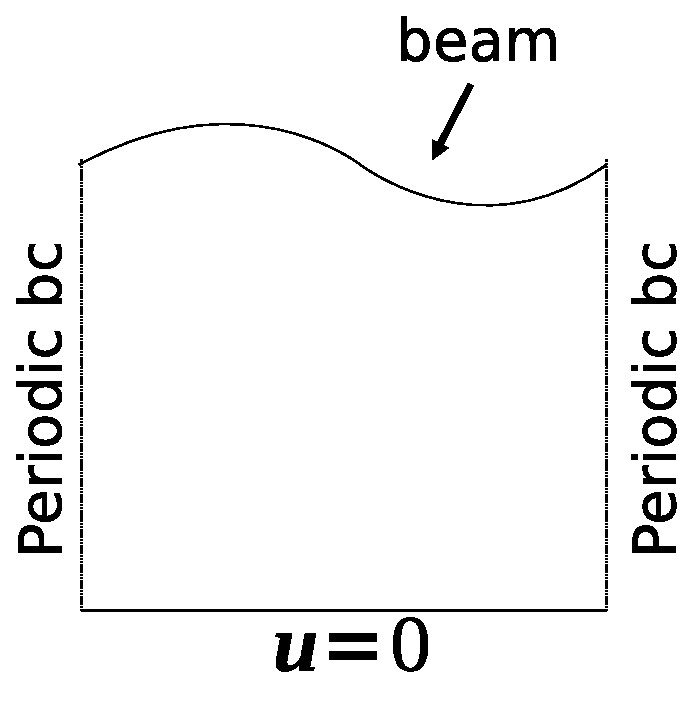
\includegraphics[width=0.5\textwidth]{exact_cartoon} 
        \caption{Geometry of the domain on which we seek an exact solution to equations (\ref{eq:100}), (\ref{eq:eq200})}
        \label{fig:ExactSolutionGeometry}.
\end{figure}
To make the problem tractable, we will assume that the inertial terms in the fluid are negligible.
The equation for the beam is 
\begin{equation} EI \frac{\partial ^4 w}{\partial x^4} = -\rho_s b h \frac{\partial ^2 w}{\partial t^2}+p(x,H)b \label{eq:100} \end{equation}
and in the fluid
\begin{equation}  \rho_f \frac{\partial u}{\partial t} = -\nabla p + \mu \nabla^2 u \label{eq:eq200} \end{equation}
The continuity condition must also be satsified.  
\[ \nabla \cdot u = 0 \]
This condition gives the pressure Poisson equation:
\begin{equation} \nabla^2 p = 0 \label{eq:eq300} \end{equation}
We will look for travelling wave solutions of the form
\begin{equation}
\begin{aligned}
w(x,t)&=\hat{w}\exp(ikx-i\omega t) \\
p(x,y,t) &= \hat{p}(y)\exp(ikx-i\omega t) \\
u_1(x,y,t) &= \hat{u}_1(y)\exp(ikx-i\omega t)\\
u_2(x,y,t) &= \hat{u}_2(y)\exp(ikx-i\omega t)
\end{aligned}
\label{eq:eq400}
\end{equation}
Plugging in these solutions, we have
\begin{equation} \begin{aligned} 
-k^2\hat{p}(y) + \hat{p}_{,yy} &= 0 \\
EIk^4\hat{w}&=\rho_s b h\omega^2\hat{w}+\hat{p}(H)b \\
-\rho i \omega \hat{u}_1+ik\hat{p}&=\mu(-k^2\hat{u}_1+\hat{u}_{1,yy}) \\
-\rho i \omega \hat{u}_2+\hat{p}_{,y}&=\mu(-k^2\hat{u}_2+\hat{u}_{2,yy}) 
\end{aligned} \label{eq:eq500}
\end{equation}
We can immediately integrate the $\hat{p}$ equation, yielding a general solution
\begin{equation} \hat{p}(y) = A\cosh{ky}+B\sinh{ky}  \label{eq:eq550} \end{equation}
Using this solution in the equation for $\hat{u}_2$, we can integrate to get
\begin{equation} \hat{u}_2(y) = M\cosh(\alpha y)+N\sinh(\alpha y)+P\cosh(k y)+Q\sinh(k y) \label{eq:eq600} \end{equation}
with 
\begin{equation} \alpha = \sqrt{-\frac{\rho_f i \omega}{\mu}+k^2}\label{eq:eq700} \end{equation}
Now applying the condition $\hat{u}_2(0)=0$ and $\hat{u}_{2,y}(0) = 0$ gives
\begin{align*}
M+P&=0\\
N\alpha+Qk&=0
\end{align*}
so that we can rewrite our solution for $\hat{u}_2$ as 
\[\hat{u}_2(y) = M\phi_1(y)+N\phi_2(y) \]
where 
\begin{equation}
\begin{aligned}
\phi_1(y) &= \frac{1}{2}\left(\cosh(\alpha y)-\cosh(k y)\right) \\
\phi_2(y) &= \frac{1}{2}\left(k\sinh(\alpha y)-\alpha\sinh(k y)\right)
\end{aligned} \label{eq:eq800}
\end{equation}
Now for this solution to satisfy the momentum equations, we must have
\begin{align*}
\frac{M}{2}\rho_f i \omega = -Bk \\
\frac{N\alpha}{2}\rho _fi \omega = -Ak
\end{align*}
So 
\begin{equation} \hat{u}_2(y) = \frac{2Bki}{\rho_f \omega}\phi_1(y)+\frac{2Aki}{\rho_f \omega \alpha}\phi_2(y)  \label{eq:eq900} \end{equation}
We must also have
\[\hat{u}_{2,y}(H) = 0 \]
so that
\[ \frac{2Bki}{\rho _f\omega}\phi_1'(H)+\frac{2Aki}{\rho_f \omega \alpha}\phi_2'(H) = 0 \]
or specifically
\[ B = -\frac{A\phi_2'(H)}{\alpha \phi_1'(H)}. \]
Then
\begin{equation} \hat{u}_2(y) = \frac{2Aki}{\rho_f \omega \alpha}\left(-\frac{\phi_2'(H)}{\phi_1'(H)}\phi_1(y)+\phi_2(y)\right)   \label{eq:eq1000} \end{equation}
The kinematic condition between the beam and the fluid is
\[ -i\omega \hat{w} = \hat{u}_2(H) \]
implying
\begin{equation} \hat{w} = -\frac{2Ak}{\rho_f \omega^2 \alpha}\left(-\frac{\phi_2'(H)}{\phi_1'(H)}\phi_1(H)+\phi_2(H)\right)   \label{eq:eq1100} \end{equation}
Finally, the beam equation in (\ref{eq:eq500}) implies 
\begin{equation} \hat{p}(H) = A\left(\cosh{kH}-\frac{\phi_2'(H)}{\alpha \phi_1'(H)}\sinh{kH}\right) \label{eq:eq1200} \end{equation}
Solvability thus requires
\[-(EIk^4-\rho_s b h\omega^2)\frac{2k}{\rho_f \omega^2 \alpha}\left(-\frac{\phi_2'(H)}{\phi_1'(H)}\phi_1(H)+\phi_2(H)\right)=\left(\cosh{kH}-\frac{\phi_2'(H)}{\alpha \phi_1'(H)}\sinh{kH}\right)b\]
This is quite a long equation.  
To simplify it, let
\[ \gamma = (EIk^4-\rho_s b h\omega^2)\frac{k}{\rho_f b} \]
Rewriting the preceding gives
\begin{equation} -\frac{2\gamma}{\omega^2 \alpha}\left(-\frac{\phi_2'(H)}{\phi_1'(H)}\phi_1(H)+\phi_2(H)\right)=\cosh{kH}-\frac{\phi_2'(H)}{\alpha \phi_1'(H)}\sinh{kH}  \label{eq:eq1300} \end{equation}
Multiplying through by $\alpha \phi_1'(H)$ gives
\[-\frac{2\gamma}{\omega^2}\left(-\phi_2'(H)\phi_1(H)+\phi_1'(H)\phi_2(H)\right)=\alpha \phi_1'(H)\cosh{kH}-\phi_2'(H)\sinh{kH}\]
Now
\begin{align*}
\phi_1'(H) &= \frac{1}{2}\left(\alpha\sinh(\alpha H)-k\sinh(k H)\right) \\
\phi_2'(H) &= \frac{k\alpha}{2}\left(\cosh(\alpha H)-\cosh(k H)\right)
\end{align*}
So
\begin{align*}
-\phi_1(H)\phi_2'(H)+\phi_2(H)\phi_1'(H)&=-\frac{\alpha k}{2}\left[1-\cosh(\alpha H)\cosh(k H)\right]-\frac{k^2+\alpha^2}{4}\sinh(kH)\sinh(\alpha H) \\
\alpha \phi_1'(H)\cosh{kH}-\phi_2'(H)\sinh{kH} &= \frac{\alpha}{2}\cosh(\alpha H)\cosh(k H) \left(\alpha\tanh(\alpha H)-k\tanh(kH) \right)
\end{align*}
So we have
\begin{equation} \frac{\gamma}{\omega^2} \frac{2\alpha k\left[1-\cosh(\alpha H)\cosh(k H)\right]+(k^2+\alpha^2)\sinh(kH)\sinh(\alpha H)} { \alpha\cosh(\alpha H)\cosh(k H) \left(\alpha\tanh(\alpha H)-k\tanh(kH) \right)} = 1 \label{eq:eq1400} \end{equation}
To make things less unwieldy, let us write the frequency $\omega$ in terms of the natural frequency of the beam, viz.,
\[ \omega = \omega_0 \tilde{\omega} \]
with
\begin{equation} \omega_0 = \sqrt{\frac{EIk^4}{\rho_s b h}} \label{eq:eq1500} \end{equation}
and
\begin{equation}  \alpha = k \sqrt{1-i\beta\tilde{\omega}} = k\eta(\tilde{\omega}) \label{eq:eq1600} \end{equation}
with
\begin{equation}   \beta = \frac{\rho_f}{\mu}\sqrt{\frac{EI}{\rho_s b h}}  \label{eq:eq1700} \end{equation}
so
\[ \gamma = \omega_0^2(1-\tilde{\omega}^2)\frac{\rho_s}{\rho_f} kh \]
Further the periodicity of the solutions in \emph{x} imply
\[ k = \frac{2n\pi}{L} \]
So that our equation becomes
 \begin{equation}  \frac{(1-\tilde{\omega}^2)}{\tilde{\omega}^2} \frac{2\eta(\tilde{\omega})\left[1-\cosh(\eta(\tilde{\omega}) kH)\cosh(k H)\right]+(1+\eta(\tilde{\omega})^2)\sinh(kH)\sinh(\eta(\tilde{\omega})kH)} { \eta(\tilde{\omega})\cosh(\eta(\tilde{\omega})k H)\cosh(k H) \left(\eta(\tilde{\omega})\tanh(\eta(\tilde{\omega})k H)-\tanh(kH) \right)} = \frac{\rho_f}{\rho_skh}  \label{eq:eq1800} \end{equation}
Note that solutions to this equation come in pairs.  Indeed, if we have a solution $\tilde{\omega}$, then $-\bar{\tilde{\omega}}$ is also a solution.  Plugging 
\[ \tilde{\omega} \mapsto -\bar{\tilde{\omega}} \]
into the afore equation gives
\[ \frac{(1-\bar{\tilde{\omega}}^2)}{\bar{\tilde{\omega}}^2} \frac{2\eta(-\bar{\tilde{\omega}})\left[1-\cosh(\eta(-\bar{\tilde{\omega}}) kH)\cosh(k H)\right]+(1+\eta(-\bar{\tilde{\omega}})^2)\sinh(kH)\sinh(\eta(-\bar{\tilde{\omega}})kH)} { \eta(-\bar{\tilde{\omega}})\cosh(\eta(-\bar{\tilde{\omega}})k H)\cosh(k H) \left(\eta(-\bar{\tilde{\omega}})\tanh(\eta(-\bar{\tilde{\omega}})k H)-\tanh(kH) \right)} = \frac{\rho_f}{\rho_skh}\]
Using the fact that $\eta(-\bar{\omega}) = \overline{\eta(\omega)}$, $\tanh(\bar{z}) = \overline{\tanh(z)}$, $\cosh(\bar{z}) = \overline{\cosh(z)}$, and $\sinh(\bar{z}) = \overline{\sinh(z)}$ demonstrates that both $\tilde{\omega}$ and $-\bar{\tilde{\omega}}$ are solutions.
Furthermore, the equation remains unchanged under the transformation
\[ k \mapsto -k \]
Then we can write our general solution for $w$ as 
\begin{align*}
w(x,t)=&\hat{w}_1 \exp(ikx-i\omega_0 \tilde{\omega} t) + \\
       & \hat{w}_2 \exp(ikx+i\omega_0 \bar{\tilde{\omega}} t) + \\
       & \hat{w}_3 \exp(-ikx-i\omega_0 \tilde{\omega} t) + \\
       & \hat{w}_4 \exp(-ikx+i\omega_0 \bar{\tilde{\omega}} t)
\end{align*}
Now for boundary conditions, we will require that the ends of the beam be pinned, so that
$w(0,t) = 0$, or namely
\begin{align*}
\hat{w}_1+\hat{w}_3=0 \\
\hat{w}_2+\hat{w}_4=0
\end{align*}
Furthermore, $w$ will only be real valued everywhere if
\begin{align*}
\hat{w}_1=\overline{\hat{w}_4} \\
\hat{w}_2=\overline{\hat{w}_3}
\end{align*}
Taking $\hat{w}_1$ real for simplicity,  we have
\begin{equation}   w(x,t) = 2\hat{w}_1\Re (\exp(ikx-i\omega_0 \tilde{\omega}t)-\exp(-ikx-i\omega_0 \tilde{\omega}t))  \label{eq:eq1900} \end{equation}
Of course, we have not explicitly enforced the moment free condition $w''(0,t) = 0$; but a simple calculation shows that it is indeed true, by a fortuitous bit of luck.
Completing the solution gives
\[\hat{u}_2(y) = -i \omega \hat{w} \left(\frac{-\phi_2'(H)\phi_1(y)+\phi_1'(H)\phi_2(y)}{-\phi_2'(H)\phi_1(H)+\phi_1'(H)\phi_2(H)}\right) \]
and
\[ \hat{u}_1(y) = -\frac{i}{k}\hat{u}_2'(y) =   \frac{\omega \hat{w}}{k} \left(\frac{-\phi_2'(H)\phi_1'(y)+\phi_1'(H)\phi_2'(y)}{-\phi_2'(H)\phi_1(H)+\phi_1'(H)\phi_2(H)}\right) \]
\begin{align*}
\hat{p}(y) &= \frac{\rho_f\omega^2\alpha^2\hat{w}}{2k}\left(\frac{\phi_2'(H)\sinh(ky)-\alpha \phi_1'(H)\cosh(ky)}{-\phi_2'(H)\phi_1(H)+\phi_1'(H)\phi_2(H)}\right)
\end{align*}
so that
\begin{equation}
p(x,y,t) = 2\Re\left[\hat{p}(y)\left(\exp(ikx-i\omega_0 \tilde{\omega}t)-\exp(-ikx-i\omega_0 \tilde{\omega}t)\right)\right]
\label{eq:eq2000} \end{equation}
and
\begin{equation}
u_2(x,y,t) = 2\Re\left[\hat{u}_2(y)\left(\exp(ikx-i\omega_0 \tilde{\omega}t)-\exp(-ikx-i\omega_0 \tilde{\omega}t)\right)\right]
\label{eq:eq2100} \end{equation}
\begin{equation}
u_1(x,y,t) = 2\Re\left[\hat{u}_1(y)\left(\exp(ikx-i\omega_0 \tilde{\omega}t)+\exp(-ikx-i\omega_0 \tilde{\omega}t)\right)\right]
\label{eq:eq2200} \end{equation}
In most practical cases, we can assume the beam is reasonably stiff, so that 
\[ \beta \gg 1 \]
Furthermore, if the fluid is light, (e.g., $\rho_s/\rho_f \gg 1$) we can approximate
\[ \tilde{\omega} \approx 1+\delta \]
where
\[ \delta \ll 1 \]
Then we can further approximate
\[ \eta(\tilde{\omega}) \approx \sqrt{-i\beta} \]
We will follow the convention
\[ \sqrt{-i\beta} = \frac{\sqrt{2}}{2}\sqrt{\beta}(1-i) \]
In this case, 
\[ \tanh(\sqrt{-i\beta}kH) \approx 1 \]
Utilizing this in the equation for $\tilde{\omega}$, and neglecting higher order terms in $\delta$, we have
\[-2\delta\left(-2\sqrt{1-i\beta}+(2-i\beta)\tanh(kH)\right) = \frac{\rho_f}{\rho_skh}(1-i\beta-\sqrt{1-i\beta}\tanh(kH)) \]
Then 
\begin{align}
\delta  &= \frac{\rho_f}{\rho_skh}\frac{1-i\beta-\sqrt{1-i\beta}\tanh(kH)}{4\sqrt{1-i\beta}-(4-2i\beta)\tanh(kH)} \nonumber \\
        &\approx -\frac{\rho_f}{2\rho_skh} \frac{2i\beta\sqrt{i\beta}-i\beta\tanh^2(kH)\sqrt{-i\beta}+\beta^2 \tanh^2 (kH)}{2\beta^2 \tanh^2 (kH)} \nonumber \\
        &\approx -\frac{\rho_f}{2\rho_skh}\left(1+\frac{\sqrt{2}}{2\sqrt{\beta}}i\right) \label{eq:eq2300}
\end{align}
where we have again taken advantage of the fact that $\beta \gg 1$. \\
{\bf Example}. \\
Consider a square domain, length and width
\begin{align*}
L = H = 0.3 \mbox{ m}
\end{align*}
and a beam with rectangular cross section, with
\begin{align*}
E &= 1.4e6 \mbox{ Pa} \\
\rho_s &= 10000 \mbox { kg/m$^3$}\\
h &= 0.02 \mbox { m} \\
I/b &= 6.67 \times 10^{-7} \mbox {m$^3$}
\end{align*}
and a fluid with properties
\begin{align*}
\rho_f &= 1000 \mbox { kg/m$^3$}\\
\nu &= 0.001 \mbox { m$^2$/s}
\end{align*}
The natural frequency of the beam is 
\[ \omega_0 = 29.9654 \mbox { rad/s} \]
We can calculate the value of $\beta$ as 
\[ \beta = 68.313005 \]
Solving for $\tilde{\omega}$ gives
\[ \tilde{\omega} =  0.8907148069 - 9.135887123 \times 10^{-3}i \]
Our approximate solution (\ref{eq:eq2300}) gives
\[ \delta = -0.1193 - 10.212 \times 10^{-3} i \]
which is somewhat off, although in this case the beam is relatively light and flexible, so our assumptions made in deriving the approximation $\delta$ are not optimal. \\
We can simulate this case in order to verify the implementation in CG and to examine the rate of convergence.  
The computation is performed on a sequence of uniform overlapping meshes of increasing refinement. 
The structure is discretized with $30$ elements in all runs. 
The max-norm errors (at $t=0.1$) and the corresponding convergence results are shown in figure \ref{fig:ExactSolutionConvergence} and table \ref{tbl:ExactSolutionConvergenceTable}.
\begin{figure}[ht]
        \centering
        \includegraphics[width=0.5\textwidth]{convergence} 
        \caption{Convergence results}
        \label{fig:ExactSolutionConvergence}
\end{figure}
\begin{table}
\centering
\begin{tabular}{ |l |  c | c| }
  \hline 
  h      & u        & v \\
  \hline 
  0.1    & 1.44(-4) & 1.03(-4) \\
  0.05   & 5.19(-5) & 3.89(-5) \\
  0.025  & 1.08(-5) & 7.87(-6) \\
  0.0125 & 2.26(-6) & 1.45(-6) \\
  \hline 
   rate   & 2.26     & 2.37 \\
  \hline 
\end{tabular}
\caption{Max-norm errors in velocity for the verification problem}
\label{tbl:ExactSolutionConvergenceTable}
\end{table}
\subsection{Compressible flow: shock hitting a flexible panel}
We can also validate our model on a compressible flow problem by running the simulation proposed by \cite{Giordano2005}.
In this simulation, a Mach 1.21 shock in air hits a $40 \mbox{ mm}$ flexible panel.  
The air is initially at $T = 293 \mbox{ K}$ and $p = 1 \times 10^5 \mbox { Pa}$.
The panel has elastic modulus $E = 220 \mbox{ GPa}$, $\nu = 0.3$, and $\rho = 7600 \mbox{ kg/m$^3$}$, and is $1 \mbox{ mm}$ thick.
A diagram describing the simulation is shown in figure \ref{fig:BeamInChannelDiagram}.
\begin{figure}[ht]
        \centering
        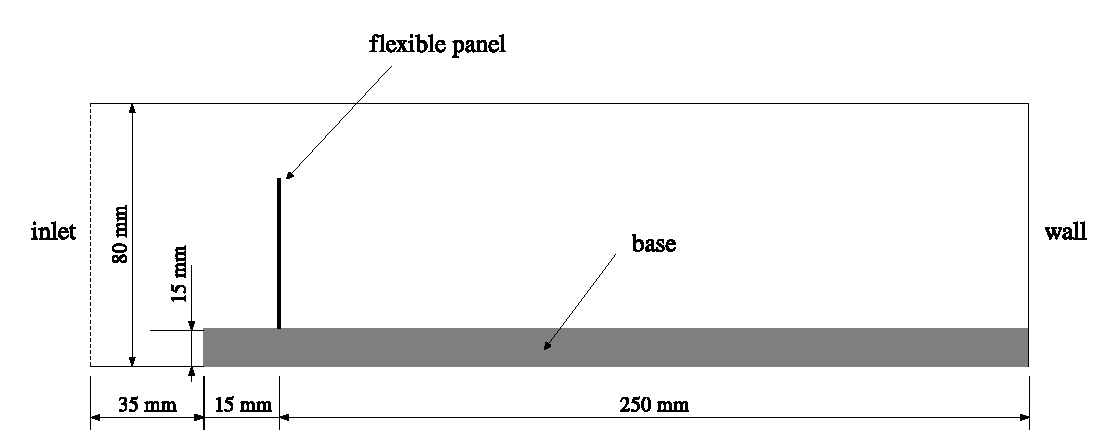
\includegraphics[width=\textwidth]{beam_in_channel_diagram} 
        \caption{Diagram describing the simulation proposed by \cite{Giordano2005}}
        \label{fig:BeamInChannelDiagram}
\end{figure}
A numerical schlieren plot is shown in figure \ref{fig:BeamInChannelSchlieren} for a time after the shock has passed the beam, showing the position of the shock wave and its reflections, as well as the vortex rollup generated by the tip of the beam.
Also visible is the deflection of the beam.
\begin{figure}[ht]
        \centering
        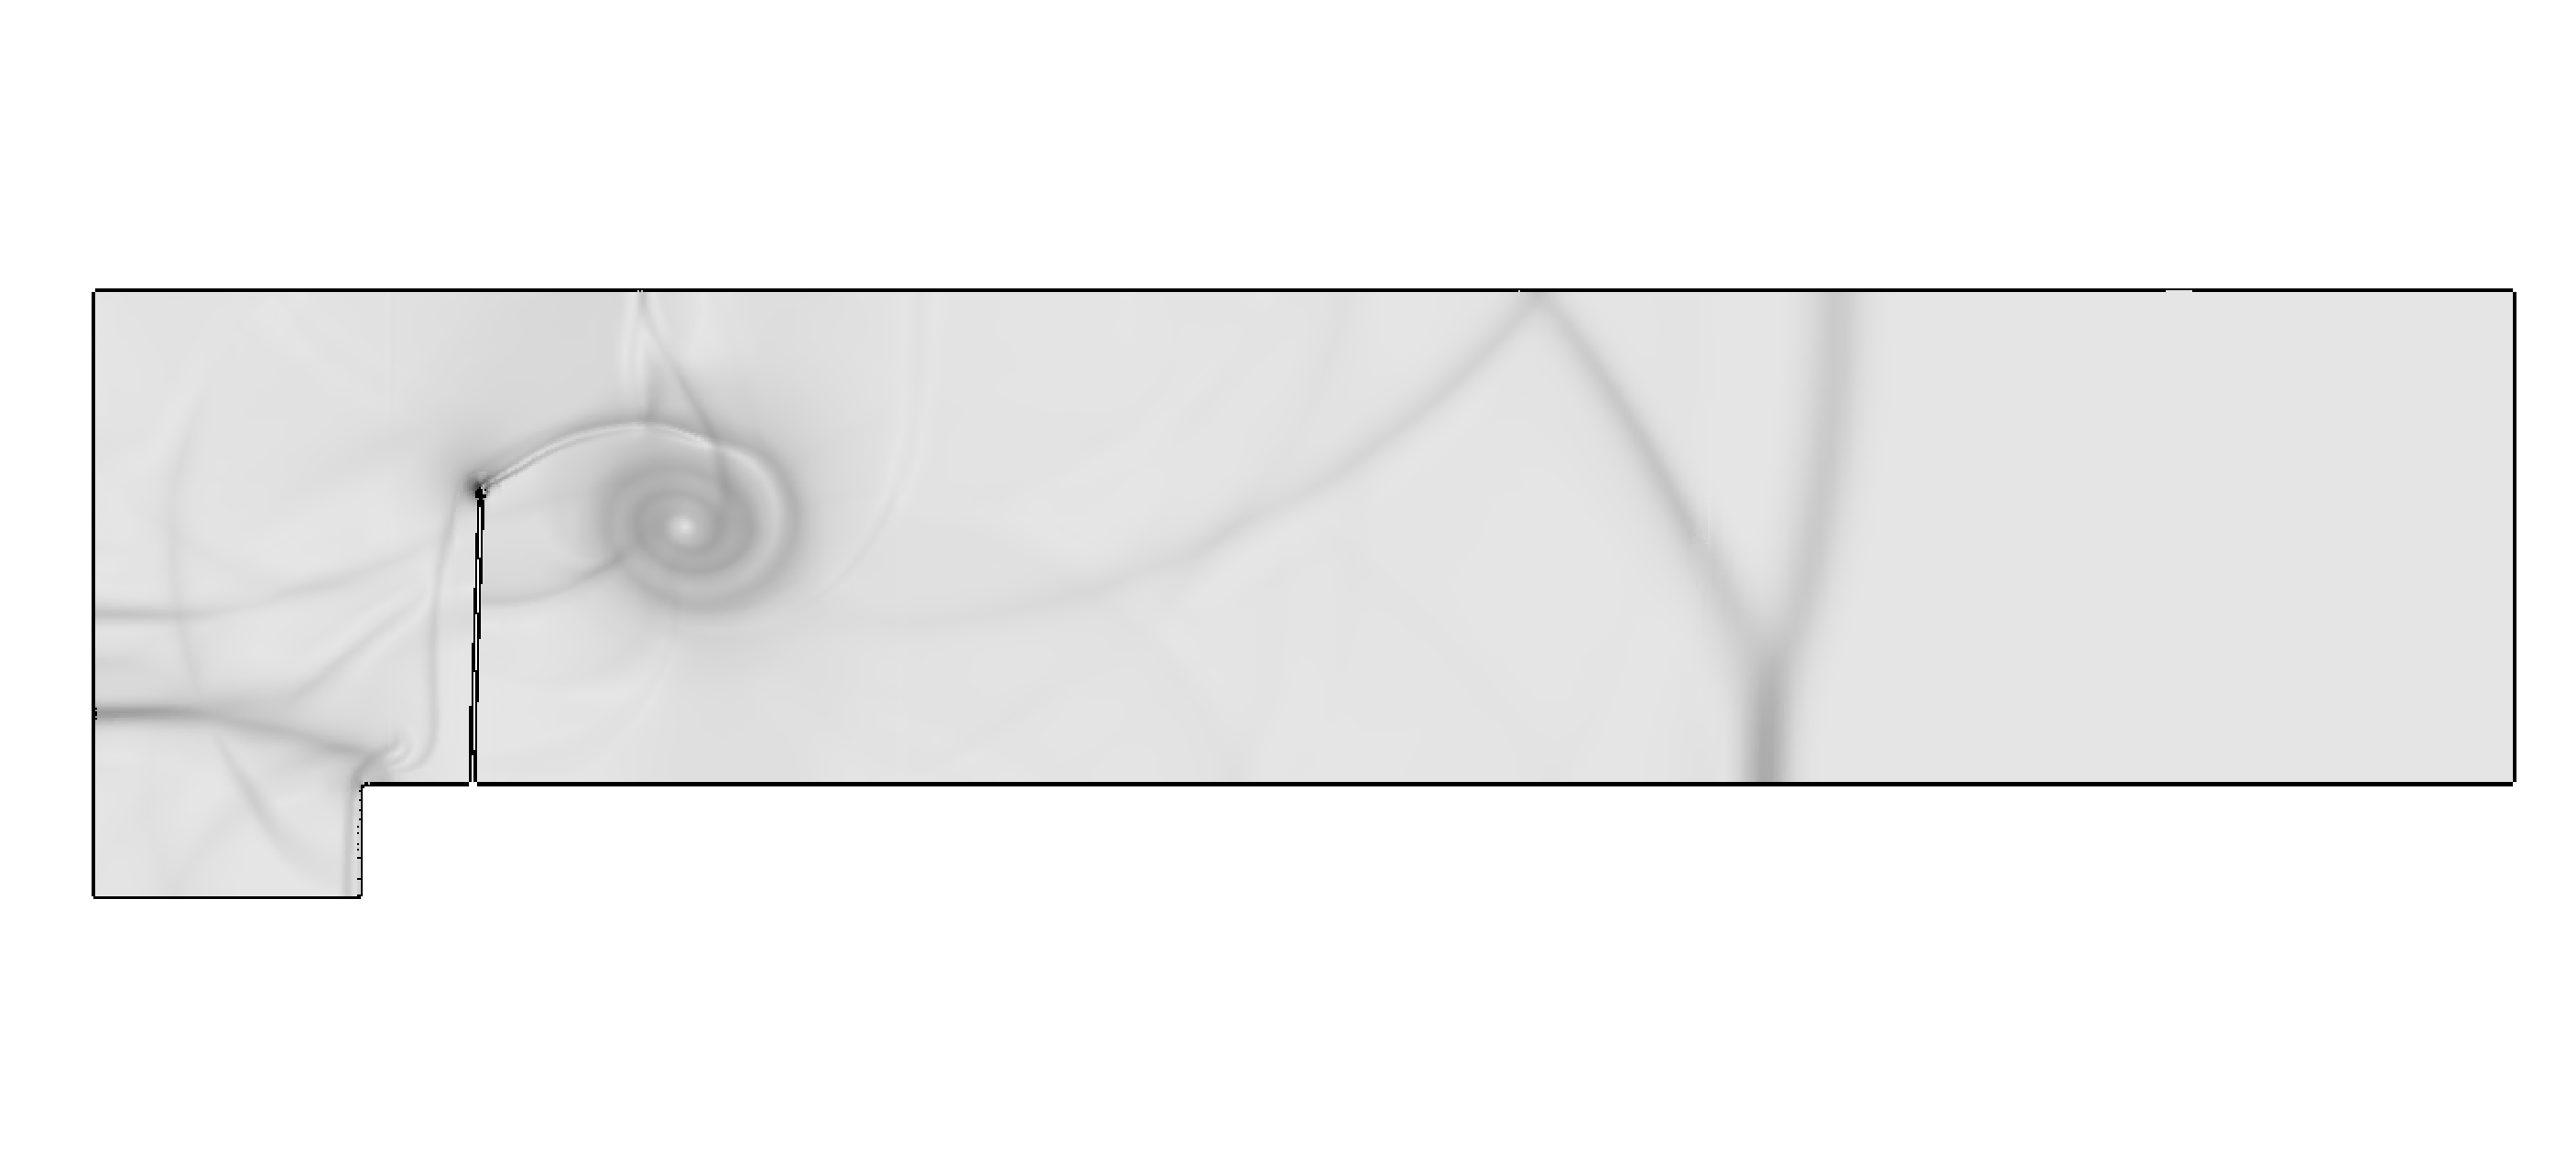
\includegraphics[width=\textwidth]{schlieren} 
        \caption{Numerical schlieren after the shock has hit the beam showing the location of the shock and the vortex rollup downstream of the beam}
        \label{fig:BeamInChannelSchlieren}
\end{figure}
A plot of the tip displacement is shown in figure \ref{fig:BeamInChannelTip1}.
Note that the times in this figure (and the succeeding ones) do not necessarily correspond (in an absolute sense) to the ones in the paper by \cite{Giordano2005}, because it is not clear from their paper how far from the step the initial shock is. 
Thus we have located it (arbitrarily) a short distance from the step.  
Of course this positioning of the shock does not affect the response beyond introducing a time shift in the results.
\begin{figure}[ht]
        \centering
        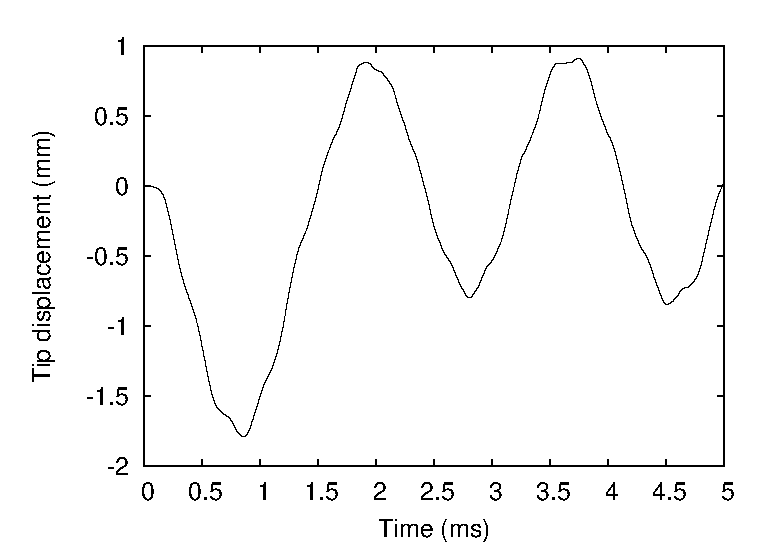
\includegraphics[width=\textwidth]{beam_in_channel} 
        \caption{Tip displacement of the panel}
        \label{fig:BeamInChannelTip1}
\end{figure}
The peak tip displacement is $1.8 \mbox{ mm}$, and the period of oscillation $1.82 \mbox{ ms}$.  
The predicted tip displacement is somewhat different than the experimental tip displacement, $2.4 \pm 0.4 \mbox{ mm}$. 
The period of oscillation predicted by our simulation is very close, however, to the measured experimental period of $1.9 \mbox{ ms}$.
To elaborate on this discrepancy, we first note that our results are mesh converged. 
A comparison of the tip displacment obtained for a fine fluid mesh and a coarse fluid mesh are shown in figure \ref{fig:BeamInChannelTip2}.
\begin{figure}[ht]
        \centering
        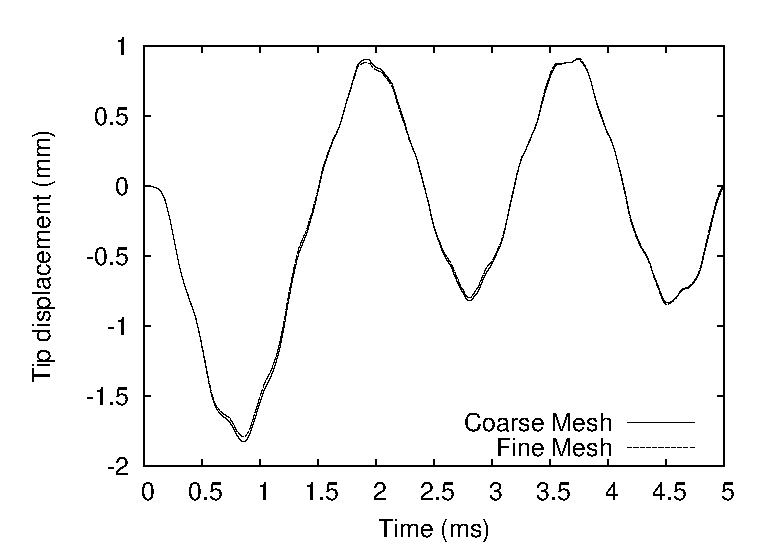
\includegraphics[width=\textwidth]{beam_in_channel2} 
        \caption{Tip displacement of the panel, demonstrating mesh convergence}
        \label{fig:BeamInChannelTip2}
\end{figure}
Further, we can compare our results to those obtained by modelling the beam as a bulk solid and running CGMP.  
To run CGMP, we had to significantly thicken the beam (to $5 \mbox{ mm}$) due to meshing considerations. 
The density and elastic modulus were reduced correspondingly to maintain the same dynamics.
The comparison is shown in figure \ref{fig:BeamInChannelTip3}.
\begin{figure}[ht]
        \centering
        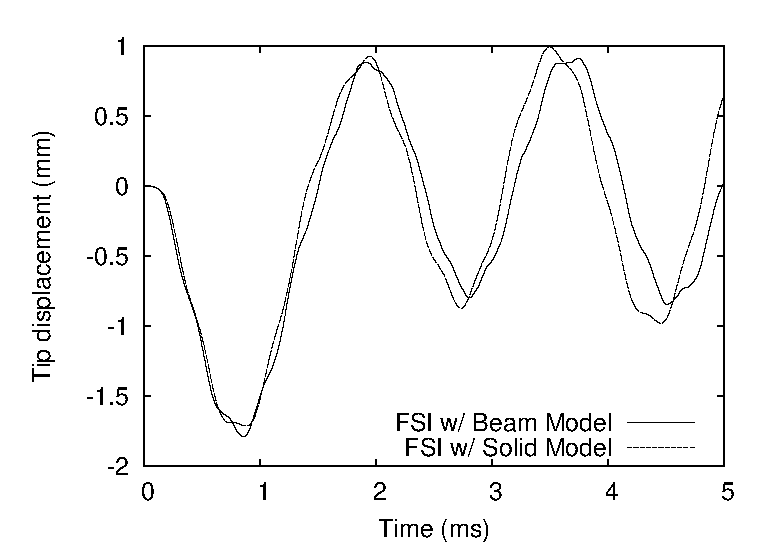
\includegraphics[width=\textwidth]{beam_in_channel3} 
        \caption{Tip displacement of the panel, comparing CGCNS + beam model and CGMP}
        \label{fig:BeamInChannelTip3}
\end{figure}
The results obtained from the new implementation and CGMP are very similar.  
The period of oscillation predicted by CGMP is slightly shorter, although this discrepancy is not surprising due to the extra thickness of the beam used in CGMP simulation.
These facts give us confidence in the correctness of our implementation.

\section{Euler-Bernoulli beam with rotation}
\subsection{Development}
Consider an Euler-Bernoulli beam, which is free to rotate.  
Let the center of mass of the beam to be located at ${\bf x}_{RB}$, and the neutral axis ${\bf \tau}$ go through this point, at an angle $\theta$.  
Let the axis normal to the beam be ${\bf n}$
We can then measure deformations of the beam with respect to this neutral axis.
Any point on the beam can then be written as 
\begin{equation} {\bf x} = {\bf x}_{RB} + {\bf n}w(\bar{x}) + {\bf t} \bar{x} \label{eq:eq6100} \end{equation}
with 
\[ \int w(\bar{x}) d\bar{x} = 0 \]
Now additionally we will require that 
\[ \int \bar{x} w(\bar{x}) d\bar{x} = 0 \] 
Then
\[ \dot{\bf x} = \dot{\bf x}_{RB} + {\bf n}(\dot{w}(\bar{x}) + \bar{x}\dot{\theta}) - {\bf t}w(\bar{x})\dot{\theta} \]
To derive the equation of motion, we can use Hamilton's principle, which says that
\begin{equation} \int_{t_1}^{t_2} \left[ \delta W_e + \delta T - \delta U + \lambda \delta w(\bar{x}) + \lambda_r \bar{x} \delta w(\bar{x}) \right] dt = 0  \label{eq:eq6200} \end{equation}
where
\begin{align*}
T &= \frac{1}{2}\rho_s b h \int |\dot{\bf x}|^2 d\bar{x}  \\
  &= \frac{1}{2}\rho_s b h \int \left[ |\dot{\bf x}_{RB}|^2 + (\dot{w}(\bar{x}) + \bar{x}\dot{\theta}) ^2 + w(\bar{x})^2\dot{\theta}^2-2\dot{\bf x}_{RB}\cdot\left( {\bf t}w(\bar{x})\dot{\theta}- {\bf n}\dot{w}(\bar{x})\right)\right] d\bar{x} \\
  &= \frac{1}{2}\rho_s b h \int \left[ |\dot{\bf x}_{RB}|^2 + (\dot{w}(\bar{x}) + \bar{x}\dot{\theta}) ^2 + w(\bar{x})^2\dot{\theta}^2 \right] d\bar{x}
\end{align*}
and
\[ U = \frac{1}{2}\int EI w''(\bar{x})^2 d\bar{x} - \rho_s b h \int {\bf g} \cdot {\bf x} d\bar{x} \]
\[ \delta W_e = \int p(\bar{x}) \delta {\bf x}\cdot{\bf n} d\bar{x} \]
Further 
\begin{align*}
\delta T = \frac{1}{2}\rho_s b h \int &\left[2 \dot{\bf x}_{RB} \cdot \delta \dot{\bf x}_{RB} + 2(\dot{w}(\bar{x}) + \bar{x}\dot{\theta}) (\delta \dot{w}+\bar{x}\delta\dot{\theta})+ \right. \\
&+\left. 2w\dot{\theta}(\delta w \dot{\theta} + w \delta \dot{\theta}) \right] d\bar{x}
\end{align*}
and 
\begin{align*}
\delta W_e &= \int p(\bar{x}) \left[ (\delta {\bf x}_{RB}\cdot {\bf n} + \bar{x}\delta \theta  + \delta w \right] d\bar{x}
\end{align*}
\begin{align*}
\delta U = &EI \int w''''(\bar{x})\delta w(\bar{x}) d\bar{x} - \rho_s b h \int {\bf g}\cdot (\delta {\bf x}_{RB}+ {\bf n} \delta w) d\bar{x} \\
           &-EI \left[ w'''(\bar{x})\delta w(\bar{x}) \right]_{-L/2}^{L/2} + EI \left[ w''(\bar{x})\delta w'(\bar{x}) \right]_{-L/2}^{L/2} 
\end{align*}
The term 
\[ EI \left[ w''(\bar{x})\delta w'(\bar{x}) \right]_{-L/2}^{L/2}  \]
is zero for clamped beams, pinned beams, and beams with free ends.  Therefore it will be dropped from here on.
The other term,
\[ -EI \left[ w'''(\bar{x})\delta w(\bar{x}) \right]_{-L/2}^{L/2} \]
is zero for free ends of beams, but non zero for beams that are pinned or clamped.  
For these beams, we can use the fact that
\[ \delta {\bf x}(\pm L/2) = \delta {\bf x}_{RB} + {\bf n}\delta w(\pm L/2) + w(L/2)(-{\bf t}\delta \theta)\pm{\bf n}\frac{L}{2}\delta \theta \]
We can enforce this condition by the use of a penalty term in the functional for $U$, so that
\[ \tilde{U} = U + \frac{1}{2}\gamma |{\bf x}(\pm L/2) - {\bf x}_0|^2 \]
and
\[ \delta \tilde{U} = \delta U + \gamma ({\bf x}(\pm L/2) - {\bf x}_0)\cdot(\delta {\bf x}_{RB} + {\bf n}\delta w(\pm L/2) + w(L/2)(-{\bf t}\delta \theta)\pm{\bf n}\frac{L}{2}\delta \theta) \]
Now denoting 
\begin{subequations}
\label{equations1}
\begin{align}
\label{eq:eq6300a}
 m &= \rho_s b h \int d\bar{x} \\
\label{eq:eq6300b}
 J &= \rho_s b h \int \bar{x}^2 d\bar{x} 
\end{align}
\end{subequations}

we must have
\begin{subequations}
\label{equations2}
\begin{align}
\label{eq:eq6400a}
 m \ddot{\bf x}_{RB} &= \int p(\bar{x}){\bf n} d\bar{x} + m {\bf g} - \gamma({\bf x}(\pm L/2) - {\bf x}_0) \\
\label{eq:eq6400b}
 J \ddot{\theta} + \int \rho_s b h\left[2\dot{w}w\dot{\theta}+w^2\ddot{\theta}\right] d\bar{x}  &= \int p(\bar{x}) \bar{x} d\bar{x} - \gamma({\bf x}(\pm L/2) - {\bf x}_0)\cdot(-w(L/2){\bf t}\pm{\bf n}\frac{L}{2}) \\
\label{eq:eq6400c}
 \rho_s b h (\ddot{w} + \bar{x}\ddot{\theta}-w\dot{\theta}^2) + EIw'''' + \lambda + \lambda_r \bar{x} &= p(\bar{x}) + \rho_s b h {\bf g} \cdot {\bf n} \\
\label{eq:eq6400d}
 w'''(\pm L/2) &= \mp \gamma({\bf x}(\pm L/2) - {\bf x}_0) \cdot {\bf n} 
\end{align}
\end{subequations}
(where $\gamma$ is taken to be zero for free ends).
Integrating the third equation, and using equation for $\ddot{\bf x}_{RB}$ (\ref{eq:eq6400a}), we must have
\begin{equation} \lambda = \frac{m}{L} \ddot{\bf x}_{RB} \cdot {\bf n} \label{eq:eq6500} \end{equation}
Likewise, we find that
\begin{equation}  \lambda_r = \frac{\rho_s b h}{J} \frac{d}{dt}\left(\rho_s b h \int w^2 \dot{\theta} d\bar{x} \right)  \label{eq:eq6600} \end{equation}
If the beam displacement is small, we can approximate 
\[ \int w^2 \dot{\theta} d\bar{x} \approx 0 \]
so that
\[ \lambda_r = 0 \]
%To come up with boundary conditions on $\ddot{w}$ for pinned/clamped beams, we can use the fact that
%\[ {\bf x}_{RB} + {\bf n}w(\pm L/2) \pm \frac{L}{2}{\bf t} = 0 \]
%\[ \dot{\bf x}_{RB} - w(\pm L/2) {\bf t}\dot{\theta} + {\bf n}\dot{w}(\pm L/2) \pm \frac{L}{2}{\bf n}\dot{\theta} = 0 \]
%\begin{align*}
%\ddot{\bf x}_{RB} + &{\bf n}\ddot{w}(\pm L/2) - {\bf t}\ddot{\theta}w(\pm L/2) - {\bf n}\dot{\theta}^2 w(\pm L/2) \\
% &-2{\bf t}\dot{\theta}\dot{w}(\pm L/2) \pm \frac{L}{2}\left({\bf n}\ddot{\theta}-{\bf t}\dot{\theta}^2\right) = 0
%\end{align*}
%Then
%\[ \ddot{\bf x}_{RB} \cdot {\bf n} + \ddot{w}(\pm L/2) - \dot{\theta}^2 w(\pm L/2)  \pm \frac{L}{2}\ddot{\theta} = 0 \]
%and
%\[ {\bf x}_{RB} \cdot {\bf n} = -w(\pm L/2) \]
%so that we can calculate
%\[ \ddot{\bf x}_{RB} \cdot {\bf n} + \ddot{w}(\pm L/2) + \dot{\theta}^2{\bf x}_{RB} \cdot {\bf n}   \pm \frac{L}{2}\ddot{\theta} = 0 \]
%which provides a means of calculating the acceleration and position of  the end of the beam at time $t^{n+1}$ once we have integrated the rigid body equations.

\subsection{Example}
As an example, consider a flexible beam falling under the influence of gravity (${\bf g} = (0,-1)$). 
The properties of the beam are
\begin{align*}
L &= 0.5 \\
h &= 0.02 \\
E &= 2 \times 10^4 \\
\rho_s &= 1 \\
I &= 6.667 \times 10^{-7}
\end{align*}
and it is initially oriented at a declination of $-30^{\circ}$ from the $x$ axis (see figure \ref{fig:FallingStick1}).  
The fluid properties are 
\begin{align*}
\nu &= 10^{-2} \\
\rho_f &= 1
\end{align*}
The inflow is at the bottom, with a parabolic profile with a maximum velocity of $v_{\mbox{in}} = 0.3$ (in the $+y$ direction).
Plots of the $y$ velocity at four representative times are shown in figures \ref{fig:FallingStick1} - \ref{fig:FallingStick4}.
Note the deflection of the beam in  \ref{fig:FallingStick4}, which is due to the build up of pressure on the underside of the beam as it is falling.
\begin{figure}[ht]
        \centering
        \subfigure[t=0]{ %{0.4\textwidth}
                \centering
                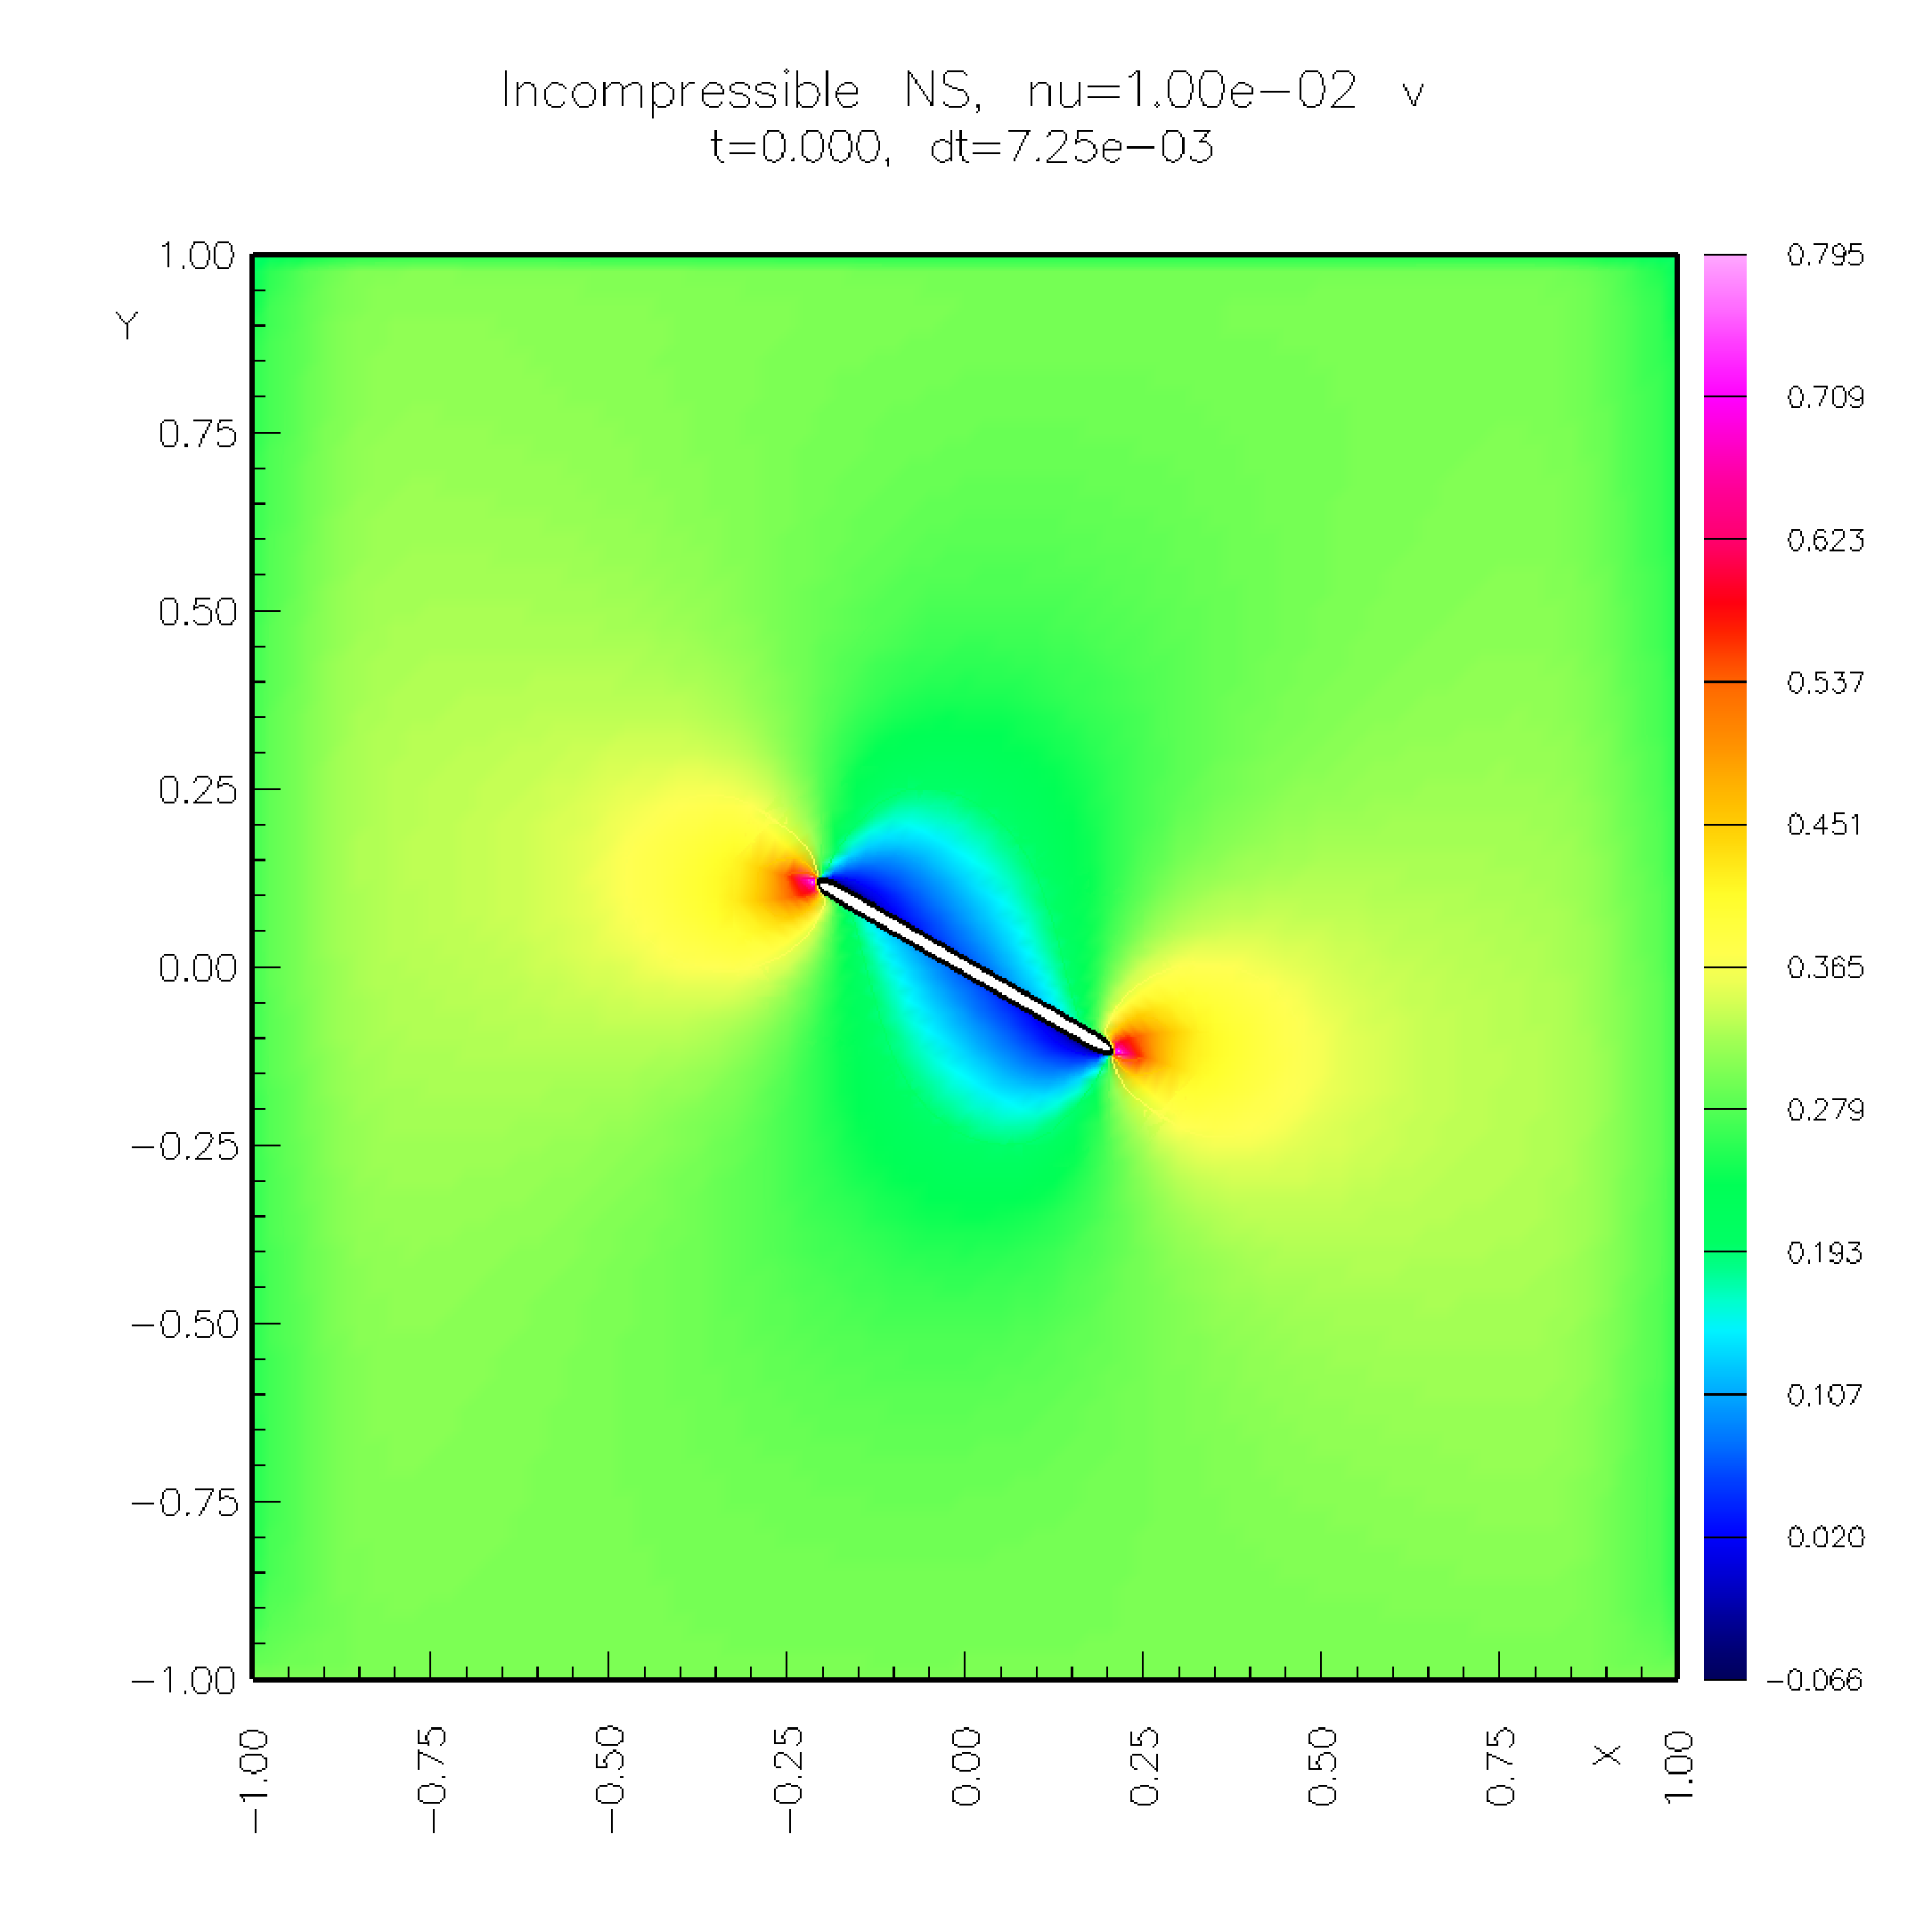
\includegraphics[width=0.4\textwidth]{fallingStick1}
                \label{fig:FallingStick1}
        }
        \subfigure[t=0.4]{%{0.4\textwidth}
                \centering
                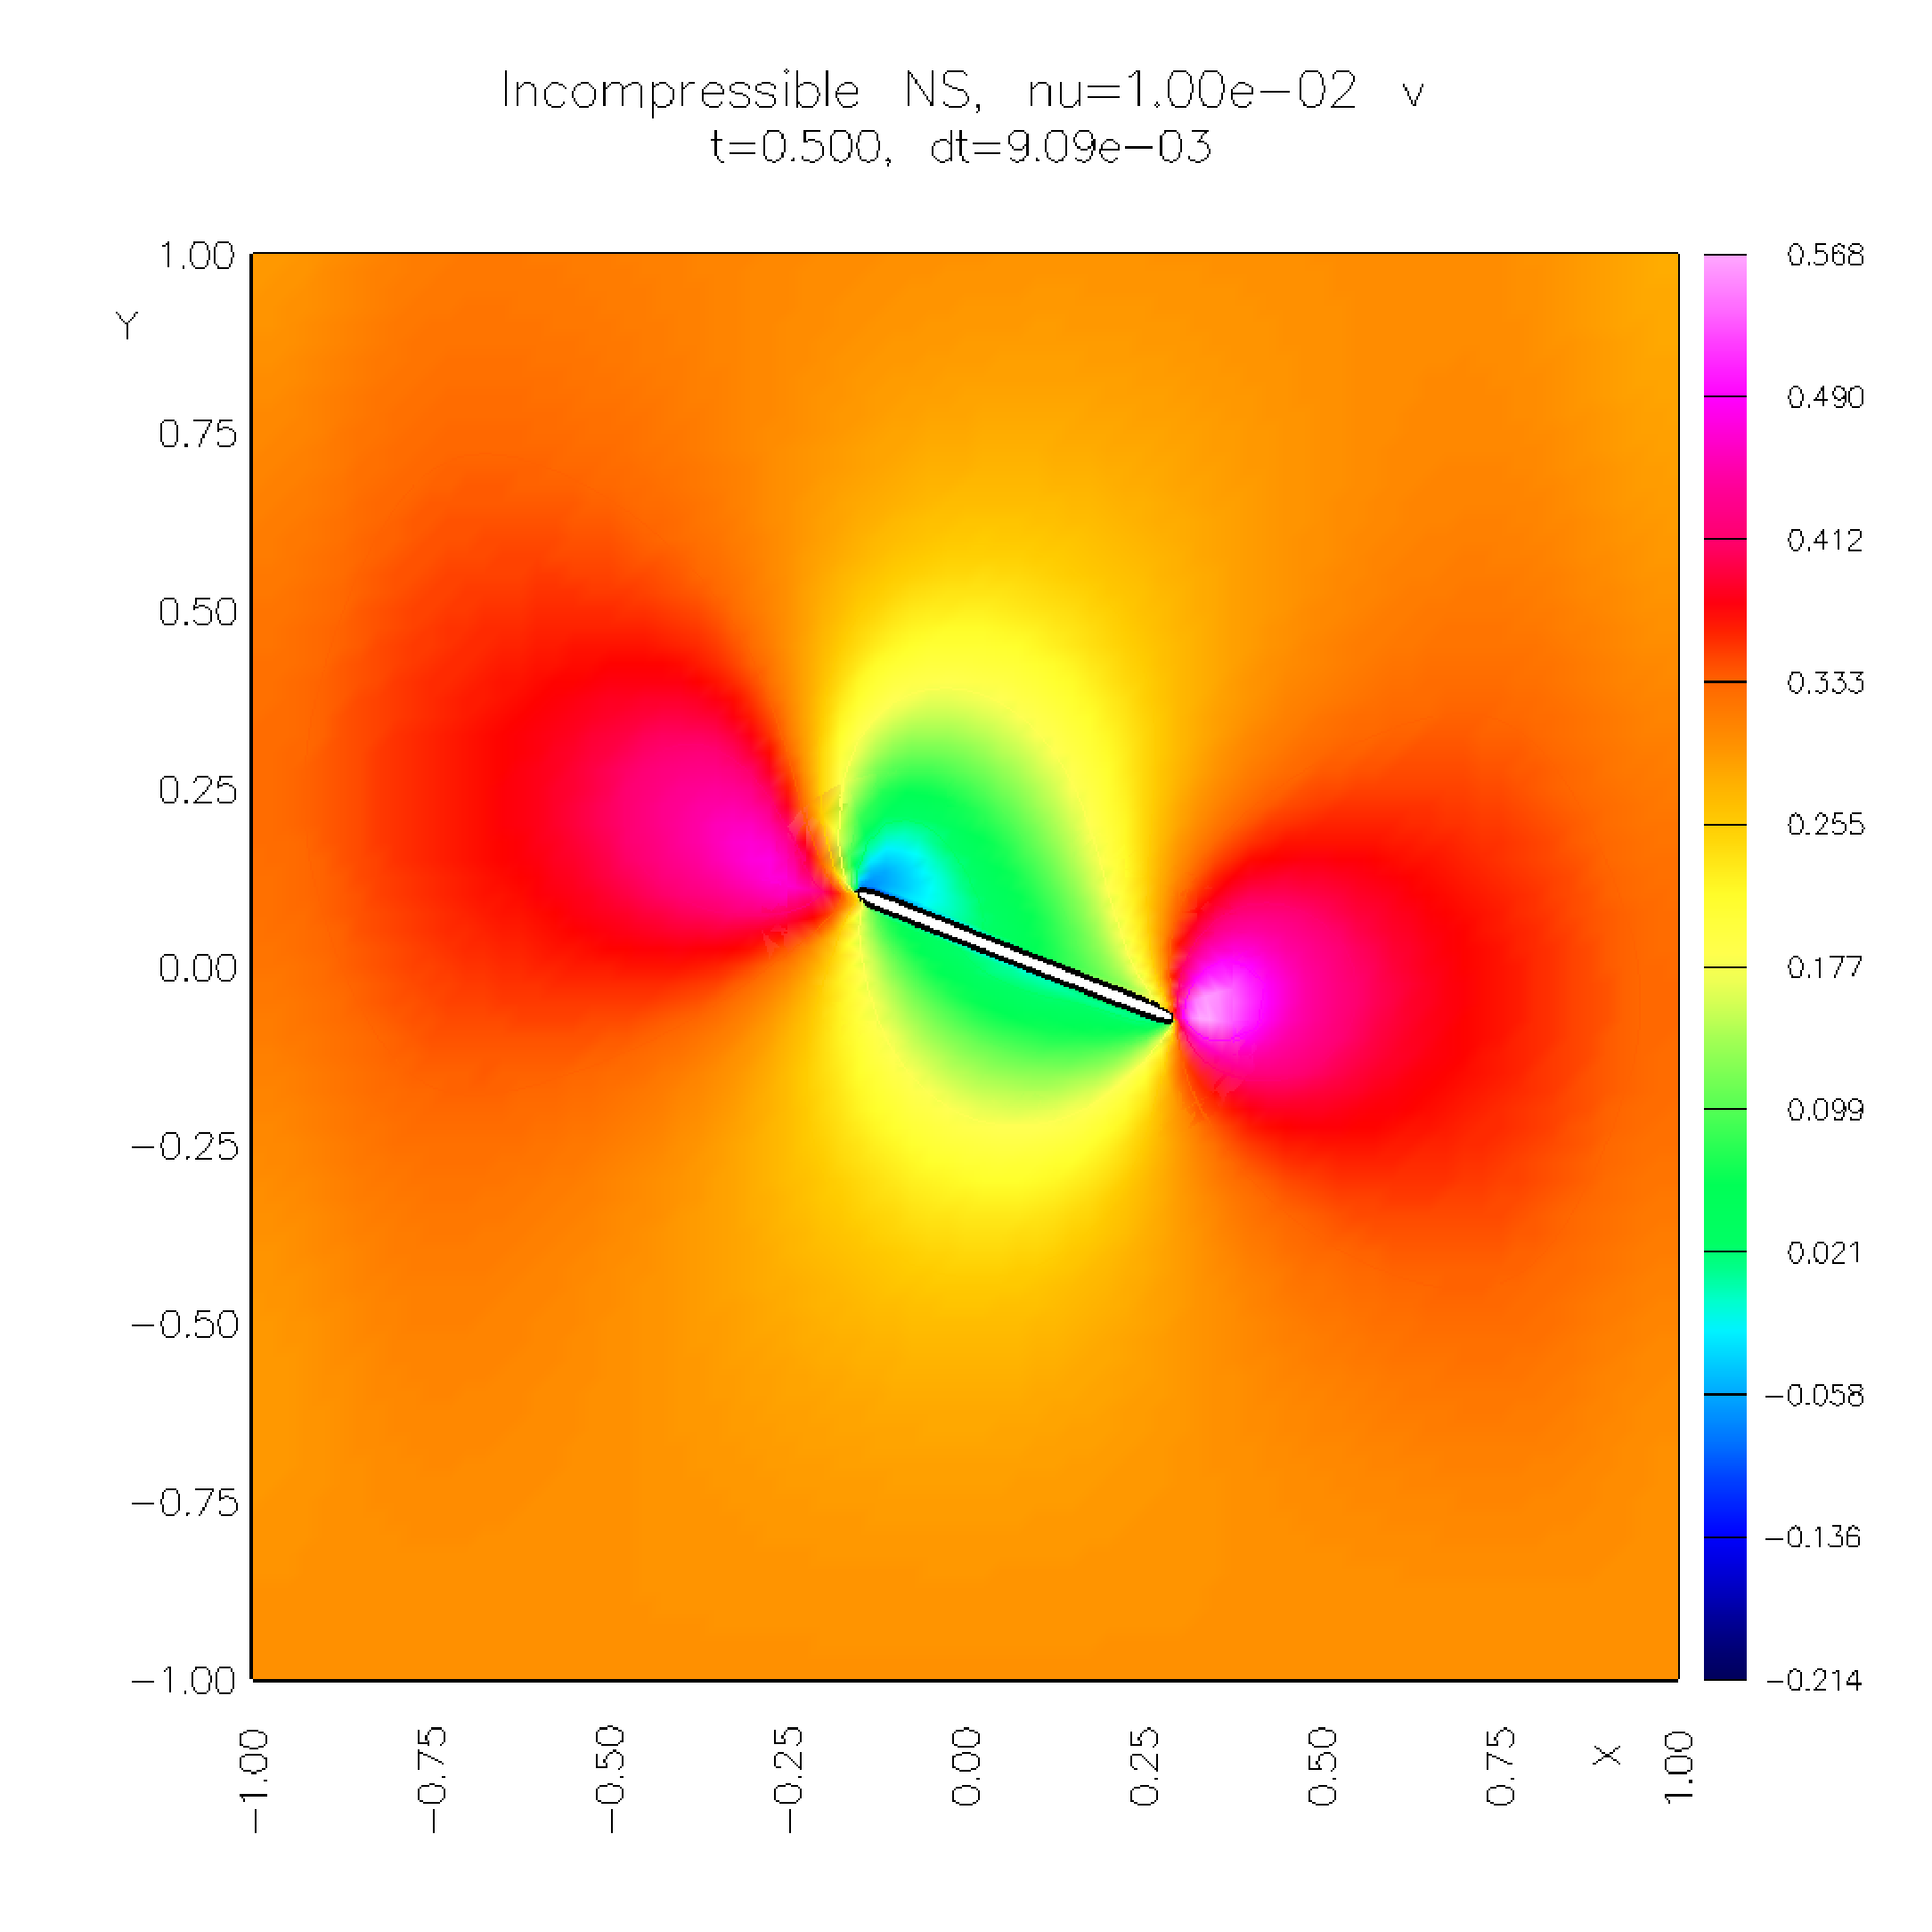
\includegraphics[width=0.4\textwidth]{fallingStick2}
                \label{fig:FallingStick2}
        } \\

        \subfigure[t=1.0]{ %{0.4\textwidth}
                \centering
                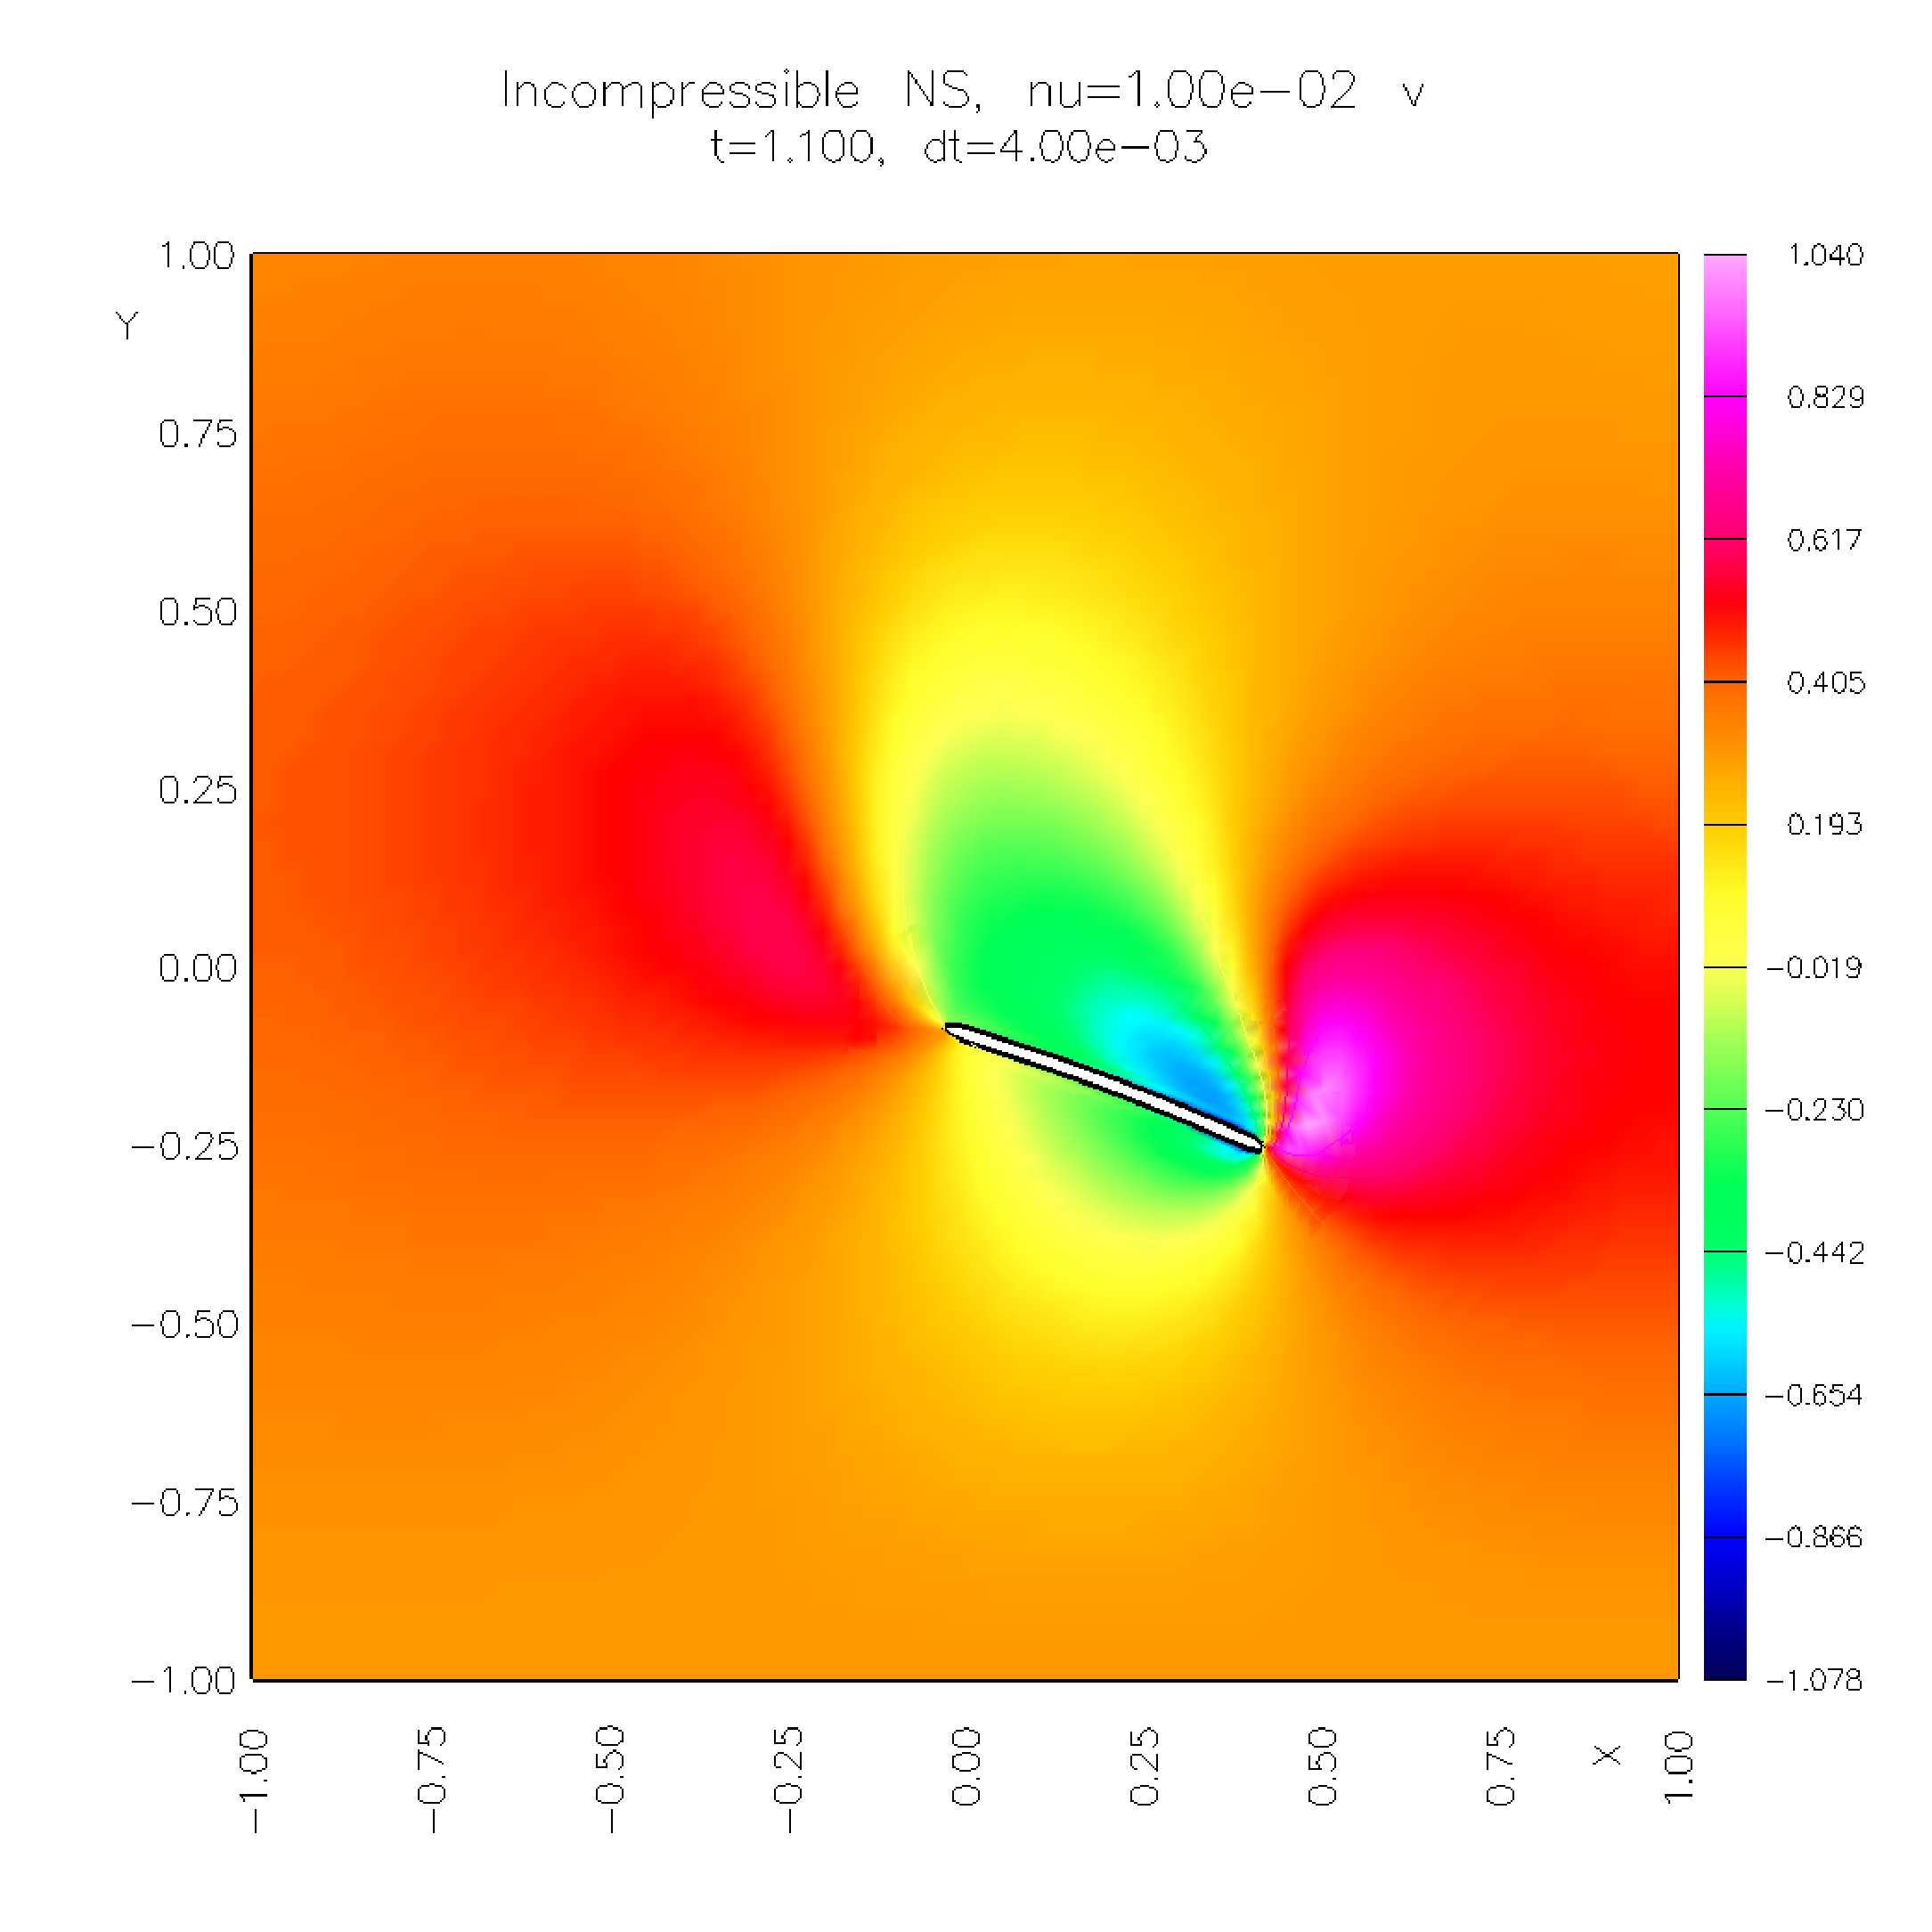
\includegraphics[width=0.4\textwidth]{fallingStick3}
                \label{fig:FallingStick3}
        }
        \subfigure[t=1.7]{%{0.4\textwidth}
                \centering
                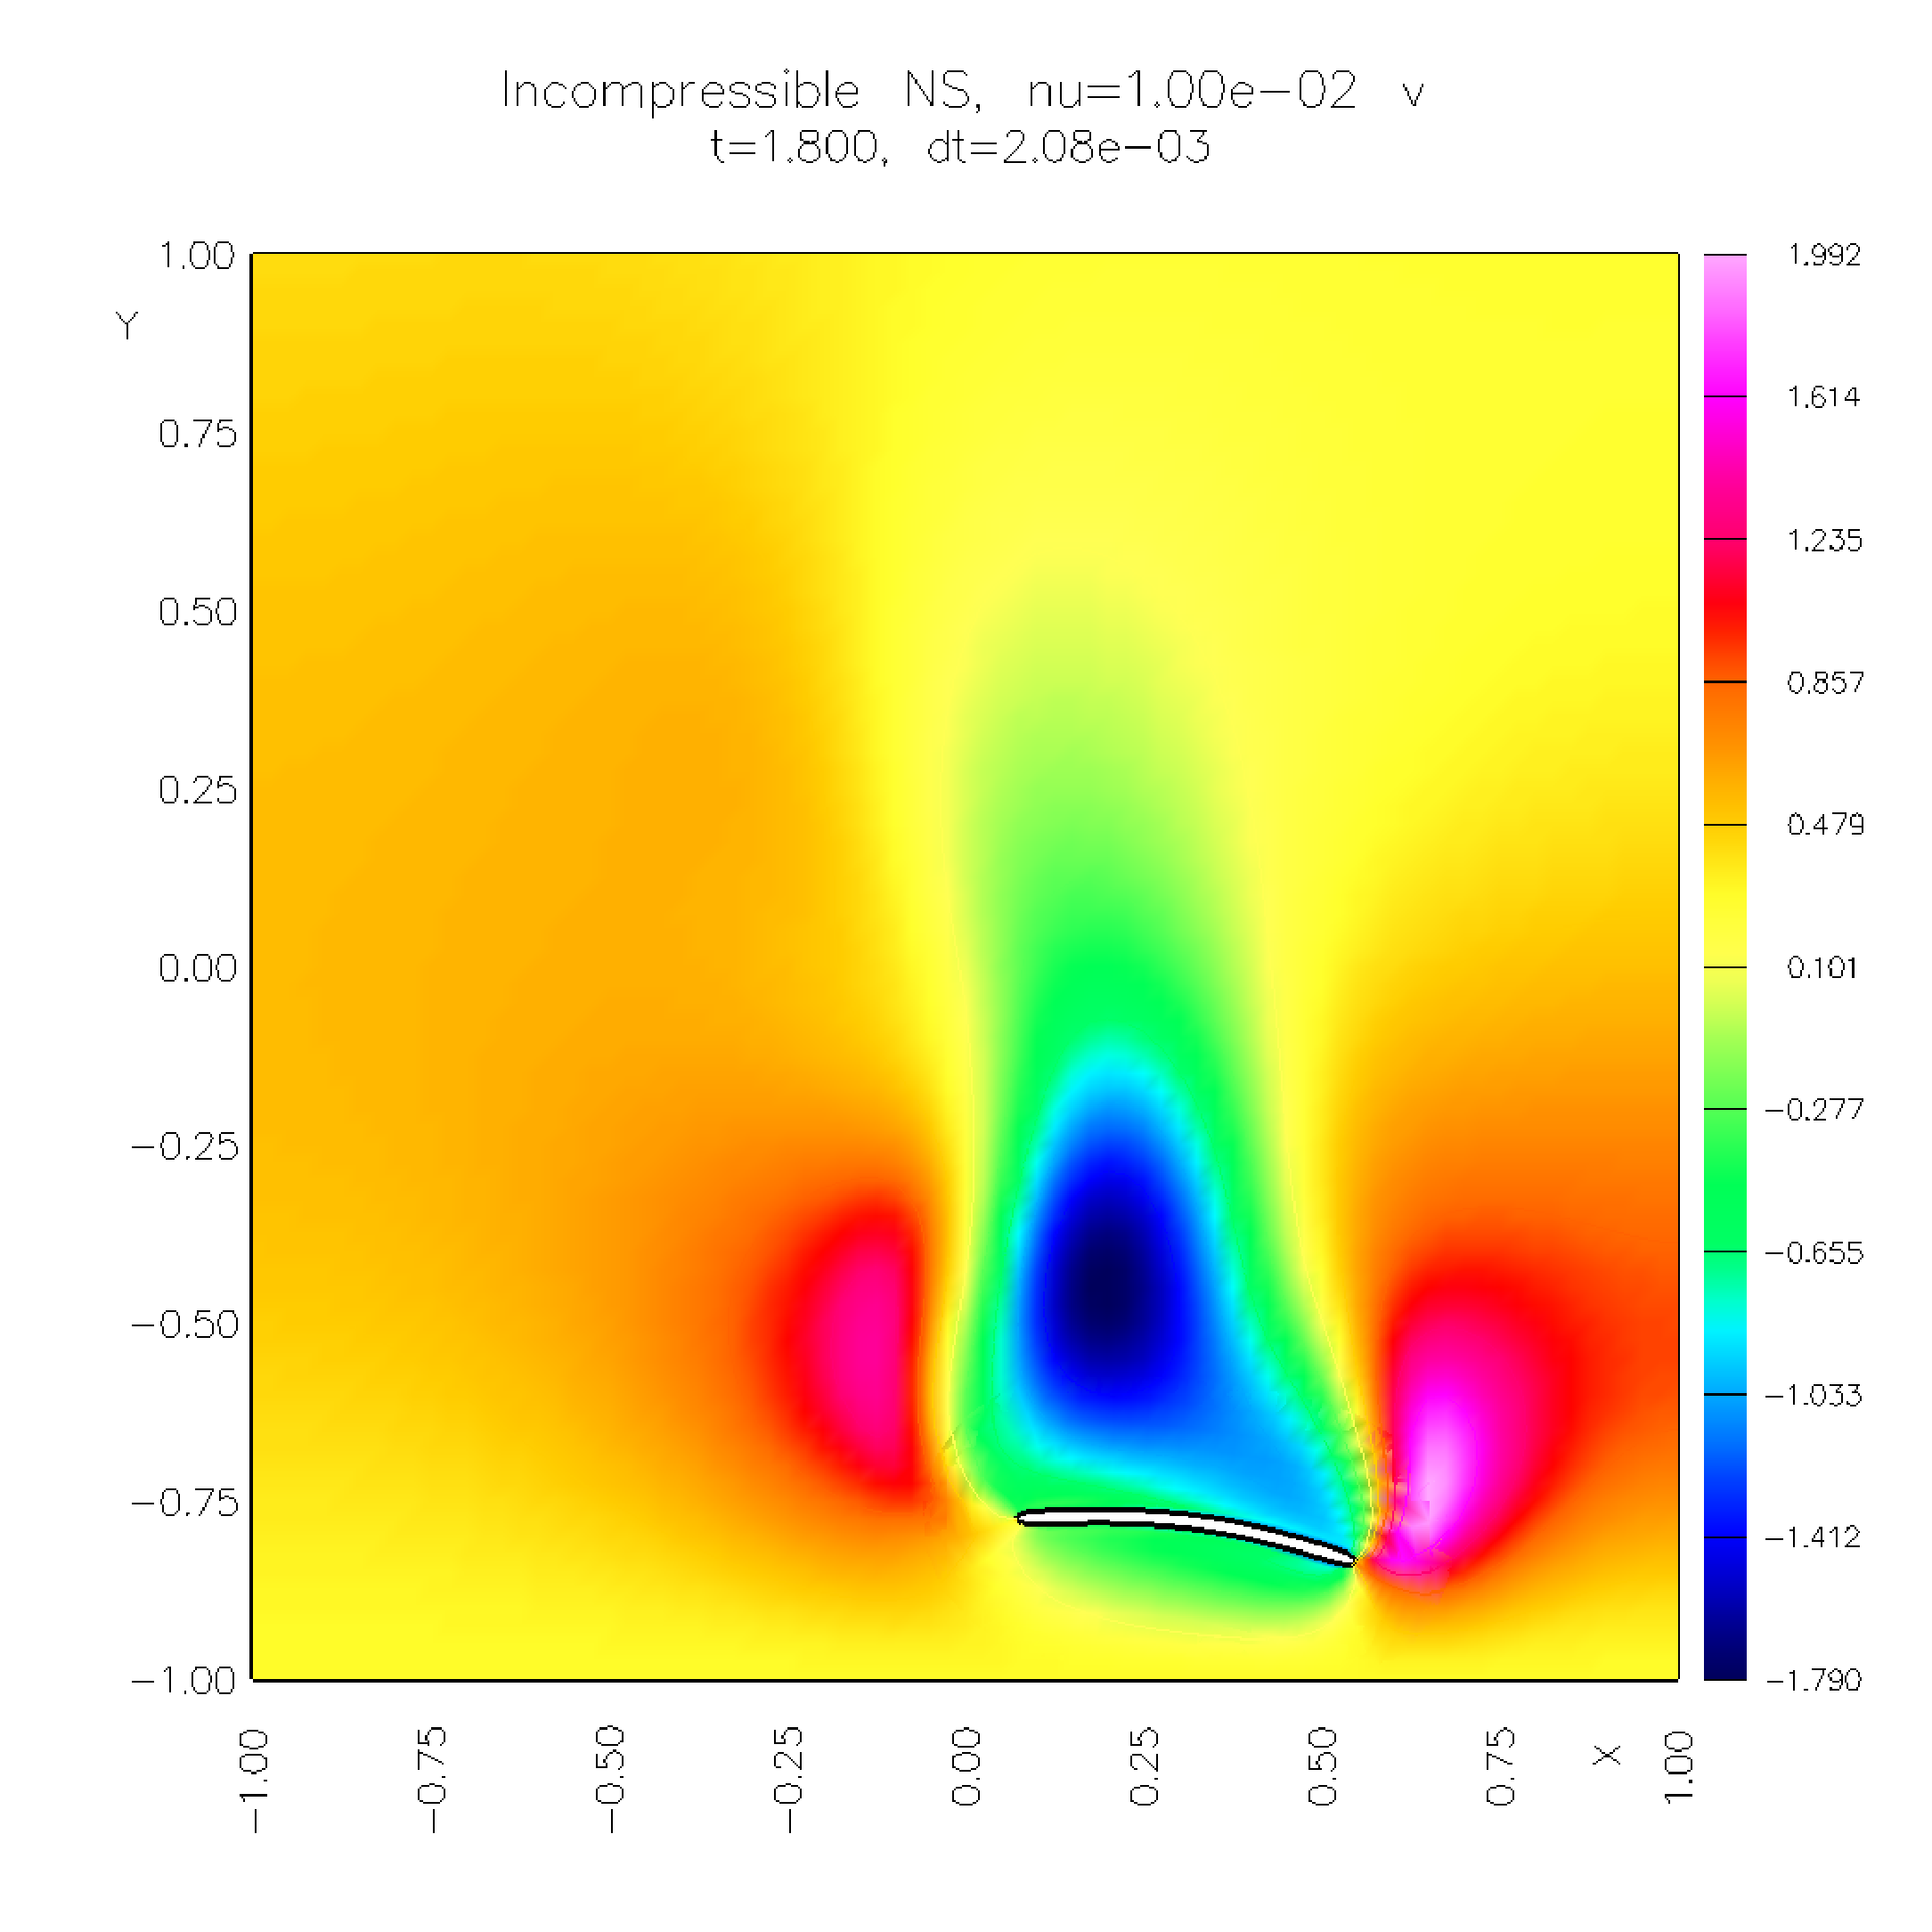
\includegraphics[width=0.4\textwidth]{fallingStick4}
                \label{fig:FallingStick4}
        }
        \caption{Contours of $y$ velocity for the falling stick test case at representative times}

\end{figure}

\section{Nonlinear beam model}
\subsection{Finite element development}
The implemented nonlinear beam model is based on the so called ``continuum based beam element'' (CB beam element).  
The basic idea of the CB beam model is to construct a beam element as a reduction of a two dimensional quad.  
Our exposition is a simplified version of the one presented by Belytschko \emph{et al}. \cite{Belytschko2000}.
The beam is defined by a set of master nodes along the center of the beam.
Associated with each master node $i$ is its location, ${\bf x}_i$, and a rotation, $\theta_i$.  
The rotation $\theta_i$ is used to define a unit vector ${\bf p}_i$, known as a director:
\begin{equation} {\bf p}_i = \cos \theta _i {\bf e}_x + \sin \theta _i {\bf e}_y \label{eq:6700} \end{equation}
The director is used to define ``slave nodes'', whose positions are
\begin{subequations}
\begin{align}
  \label{eq:eq6800a}
 {\bf x}_i^+ &= {\bf x}_i + \frac{h_i}{2}{\bf p}_i  \\
  \label{eq:eq6800b}
 {\bf x}_i^- &= {\bf x}_i - \frac{h_i}{2}{\bf p}_i 
\end{align}
\end{subequations}

where $h_i$ is the thickness of the beam at node $i$.
These slave nodes are used to construct the quads needed for the CB beam approximation.
In particular, the two noded beam element defined by nodes $i$, $i+1$ has an associated four noded quad whose nodes are (in counter-clockwise order):
\[ {\bf x}_i^-, {\bf x}_{i+1}^-,  {\bf x}_{i+1}^+, {\bf x}_i^+ \]
It is possible to construct beam elements with three (or more) nodes, but the elements used herein are two-noded beams and their associated four-noded quads.
Following Belytschko, we use a (primarily) updated Lagrangian formulation.  
The general form of the internal nodal force at a node $I$ in this formulation in a slave element whose domain is $\Omega$ is
\begin{equation} {\bf f}_I^{\mbox{int}} = \int _{\Omega} \left[ N_{I,x} \ N_{I,y} \right] {\boldsymbol \sigma} d\Omega \label{eq:eq6900} \end{equation}
where $N_I$ is the shape function associated with node $I$.  
This integral is done using Gaussian quadrature.  
Let use natural coordinates $(\xi, \eta)$ for our quad.  
In order to avoid locking, only one quadrature point is used in the direction along the beam axis (at $\xi = 0$), with multiple points (e.g., 3) in the $\eta$ direction.  
Then we can approximate
\begin{equation}  {\bf f}_I^{\mbox{int}} = \frac{h}{h_0} \sum_{i=1}^{n_Q}  \left[N_{I,x} \ N_{I,y}\right] {\boldsymbol \sigma} J_{\xi} w_i b_i \label{eq:eq7000} \end{equation}
where $w_i$ are the quadrature weights, $b_i$ is the beam width at the quadrature point location, and $J_{\xi}$ is the Jacobian of the map from the element natural coordinates to global coordinates. 
The extra term $h/h_0$ is, to quote Belytschko, ``a factor that accounts approximately for the change in thickness''. 
On an element with nodes $i$, $i+1$, I use 
\begin{equation} \frac{h}{h_0} \approx \frac{1}{2}\|{\bf p}_i + {\bf p}_{i+1} \| \label{eq:eq7100} \end{equation}
Now the key to the beam approximation is the assumption that the normal stress perpendicular to the axis of the beam is zero.  
This must be enforced explicitly in the computation of the internal force.  
To do this, let us define what is called a \emph{laminar} coordinate system at each quadrature point.  
The basis vector $\hat{\bf e}_x$ for this system is defined to be tangent to lines of constant $\eta$.  
The basis vector $\hat{\bf e}_y$ is then perpendicular to  $\hat{\bf e}_x$.
Now further let 
\begin{equation} {\bf R} = \begin{bmatrix}
\hat{\bf e}_x \cdot {\bf e}_x & \hat{\bf e}_y \cdot {\bf e}_x \\
\hat{\bf e}_x \cdot {\bf e}_y & \hat{\bf e}_y \cdot {\bf e}_y
\end{bmatrix}
 \label{eq:eq7200} \end{equation}
Note that we construct a new coordinate system $\hat{\bf e}_x$,$\hat{\bf e}_y$ at each quadrature point.
Then we can rewrite ${\bf f}_I^{\mbox{int}}$ as 
\begin{equation}  {\bf f}_I^{\mbox{int}} = \frac{h}{h_0} \sum_{i=1}^{n_Q}  \left[ N_{I,\hat{x}} \ N_{I,\hat{y}}\right] \hat{ \boldsymbol \sigma  } {\bf R}^T J_{\xi} w_i b_i 
 \label{eq:eq7300} \end{equation}
Now we enforce normal stress perpendicular to the axis of the beam is zero by setting $\sigma_{\hat{y}\hat{y}} = 0$, so that
\begin{equation} \hat{ \boldsymbol \sigma  } = \begin{bmatrix}
\sigma_{\hat{x}\hat{x}} & \sigma_{\hat{x}\hat{y}} \\
\sigma_{\hat{x}\hat{y}} & 0
\end{bmatrix} \label{eq:eq7400} \end{equation}
In this basis, we can also compute the deformation gradient 
\begin{equation} \hat {\bf F} = \frac{\partial \hat{\bf x}}{\partial \hat{\bf X}} \label{eq:eq7500} \end{equation}
and the Green-Lagrange strain
\begin{equation} \hat {\bf E} = \frac{1}{2}\left( \hat {\bf F}^T \hat {\bf F} - {\bf I} \right) \label{eq:eq7600} \end{equation}
Now generally we have some constituitive law that maps
\[ \hat {\bf E} \to  \hat{ \boldsymbol \sigma  }  \]
But of course now we have a problem, because $ \hat {\bf E} $  has three degrees of freedom, but $\hat{ \boldsymbol \sigma  } $ only two!
We get around this problem by modifying the tensor $\hat {\bf E}$ so that we can maintain $\sigma_{\hat{y}\hat{y}} = 0$.  
Consider the isotropic SVK material law:
\begin{equation} {\bf S} = \lambda \mbox{tr} {\bf E} + 2\mu {\bf E}  \label{eq:eq7700} \end{equation}
We assume that the beam is in a state of plane stress, so that
\[ {\sigma}_{\hat{x}\hat{z}} = {\sigma}_{\hat{y}\hat{z}} = {\sigma}_{\hat{z}\hat{z}} = 0 \]
Now let $\tilde{\bf e}_x$, $\tilde{\bf e}_y$ be a basis aligned with the beam (so that $\tilde{\bf e}_x$ points along the axis of the beam) in the undeformed configuration.
Further let ${\bf R}_{\mbox{def}}$ be a rotation matrix from the $\tilde{\bf e}_x$, $\tilde{\bf e}_y$ basis to the $\hat{\bf e}_x$,$\hat{\bf e}_y$  basis.
Then 
\begin{equation} \tilde{\bf E} = {\bf R}_{\mbox{def}} \hat {\bf E} {\bf R}_{\mbox{def}}^T  \label{eq:eq7800} \end{equation}
Now in the continuum beam model, it is the component $\tilde{E}_{yy}$ we will modify to enforce $\sigma_{\hat{y}\hat{y}} = 0$.
Writing the stress in terms of the Piola-Kirchhoff stress and the deformation gradient, we have
\begin{equation} \hat{ \boldsymbol \sigma  } = \frac{1}{J(\partial z / \partial Z)^2}\hat{\bf F} \hat{\bf S} \hat{\bf F}^T  \label{eq:eq7900} \end{equation}
where $J = \det{\bf F}$, and 
\begin{equation} (\partial z / \partial Z) = \sqrt{1-2\frac{\nu S_{\hat{x}\hat{x}}}{E}} \label{eq:eq8000} \end{equation}
is a term to approximately correct for the deformation of the beam in the $y$ and $z$ directions. 
Note that there is still an inconsistency between ${\bf F}$ and ${\bf E}$  (because we have have modified ${\bf E}$); in theory we could have modified ${\bf F}$ to begin with, but it is not immediately obvious which components to modify.
Further, we have already made some modelling assumptions.
Then we have 
\begin{equation} \hat{ \boldsymbol \sigma  } = \frac{1}{J(\partial z / \partial Z)^2}\hat{\bf F} {\bf R}_{\mbox{def}}^T \left(\lambda \mbox{tr} \tilde{\bf E} + 2\mu \tilde{\bf E}\right){\bf R}_{\mbox{def}}  \hat{\bf F}^T  \label{eq:eq8100} \end{equation}
Now this is a set of six linear equations, in which our unknowns are $\sigma_{\hat{x}\hat{x}}$, $\sigma_{\hat{x}\hat{y}}$, $\tilde{E}_{yy}$,$\tilde{E}_{xz}$,$\tilde{E}_{yz}$, and $\tilde{E}_{zz}$.
Hence we can solve for the unknowns, and thereby compute the stress tensor.

After obtaining the nodal forces at the slave nodes, we must transform them in order to obtain the forces at the master nodes.
This is done by a simple transformation:
\begin{equation} {\bf f}_{\mbox{master,I}} = \left[ \begin{array}{c} f_I^x \\ f_I^y \\ m_I \end{array} \right] = {\bf T}_I^T \left[ \begin{array}{c} f_{I-}^x \\  f_{I-}^y \\ f_{I+}^x \\  f_{I+}^y \end{array} \right]  \label{eq:eq8200} \end{equation}
where $ \left[ f_{I-}^x \ f_{I-}^y \right]$ is the nodal force at the slave node $(-)$ corresponding to master node $i$ (and likewise for slave node $(+)$), and 
\begin{equation} {\bf T} = \begin{bmatrix} 
1 & 0 & y_I - y_I^- \\
0 & 1 & x_I^- - x_I \\
1 & 0 & y_I - y_I^- \\
0 & 1 & x_I^+ - y_I 
\end{bmatrix} \label{eq:eq8300} \end{equation}
The mass matrix can be written as a transformation of the mass matrix of the two-dimensional quad. 
Denoting this mass matrix as ${\bf M}^{\mbox{slave}}_e$, we define (per Belytschko)
\begin{equation} {\bf M}_e = {\bf T}_e^T {\bf M}^{\mbox{slave}}_e  {\bf T}_e  \label{eq:eq8400} \end{equation}
where
\begin{equation}  {\bf T}_e =  \begin{bmatrix}  
{\bf T}_I &  \\
            & {\bf T}_{I+1} 
\end{bmatrix}  \label{eq:eq8500} \end{equation}
To compute the inertial force, we first note that we must have
\begin{equation}  {\bf f}^{\mbox{inertia}}_{e, \mbox{master}} = {\bf T}_e^T{\bf f}_{e, \mbox{slave}} \label{eq:eq8600} \end{equation}
Now 
\begin{align}
{\bf f}^{\mbox{inertia}}_{e, \mbox{slave}} &= \frac{d}{dt}\left({\bf M}^{\mbox{slave}}_e \dot{\bf u}_{e,\mbox{slave}} \right) \nonumber \\
                          &= \frac{d}{dt}\left({\bf M}^{\mbox{slave}}_e {\bf T}_e \dot{\bf u}_{e,\mbox{master}} \right)
 \label{eq:eq8700}
\end{align}
where 
\[ {\bf u}_{e,\mbox{master}} = \begin{bmatrix}  x_I \\ y_I \\ \theta_I \\ x_{I+1} \\ y_{I+1} \\ \theta_{I+1} \end{bmatrix} \]
and
\[ {\bf u}_{I,\mbox{slave}} = \begin{bmatrix}  x_I^- \\ y_I^- \\  x_I^+ \\ y_I^+ \\ x_{I+1}^- \\ y_{I+1}^- \\  x_{I+1}^+ \\ y_{I+1}^+ \end{bmatrix} \]
Now Belytschko suggests neglecting the dependence of ${\bf T}_e$ on time, so that
\[ {\bf f}^{\mbox{inertia}}_{e, \mbox{master}} = {\bf M}_e \ddot{\bf u}_{e,\mbox{master}} \] 
However, I found that this causes the rotational degrees of freedom to become unstable.
Therefore, I use the correct expression for the inertial force,
\begin{equation}  {\bf f}^{\mbox{inertia}}_{e, \mbox{master}} = {\bf M}_e \ddot{\bf u}_{e,\mbox{master}} + {\bf T}_e^T {\bf M}^{\mbox{slave}}_e \dot{\bf T}_e \dot{\bf u}_{e,\mbox{master}}\label{eq:eq8800} \end{equation} 
$\dot{\bf T}_e$ can be formed by noting that
\begin{equation}  \dot{\bf T}_e = \dot{\theta}_I \begin{bmatrix} 
0 & 0 & x_I - x_I^- \\
0 & 0 & y_I - y_I^- \\
0 & 0 & x_I - x_I^+ \\
0 & 0 & y_I - y_I^+ 
\end{bmatrix} \label{eq:eq8900} \end{equation} 
The element stiffness matrix (in the deformed coordinate system) can be written as the sum of two parts, material and geometric.
For the material stiffness, we note that in a reference configuration
\begin{equation}  {\bf K}^{\mbox{mat}}_{IJ} = \int_{\Omega_0} {\bf B}_0^T {\bf C}_0^{SE}   {\bf B}_0 d\Omega_0 \label{eq:eq9000} \end{equation} 
where ${\bf C}^{SE}$ are the tangent moduli, (so that $\dot{\bf S} = {\bf C}^{SE} : \dot{\bf E} $) and 
${\bf B}$ is the standard matrix relating the displacement vector to strains in the reference configuration.
Now we must have again $\sigma_{\hat{y}\hat{y}} = 0$ and therefore 
\[ \frac{D\sigma_{\hat{y}\hat{y}}}{Dt} = 0 \]
Theoretically, we should enforce this condition by choosing ${\bf C}^{SE}$ so that this condition is satisfied.
In practice, I just approximate this condition with
\[ \dot{\bf S}_{\hat{y}\hat{y}} = 0 \]
which seems to work well.
Then if we take the deformed configuration to be instantaneously the reference configuration we have
\begin{equation}   \hat{{\bf K}}^{\mbox{mat}}_{e,IJ} = \int_{\Omega} {\bf B}_{I*}^T {\bf C}^{\mbox{lam}}   {\bf B}_{J*} d\Omega \label{eq:eq9100} \end{equation} 
where 
\begin{equation}   {\bf B}_{I*} = \begin{bmatrix}
N_{I, \hat{x}} & 0  \\
N_{I, \hat{y}} & N_{I, \hat{x}}
\end{bmatrix}  \label{eq:eq9200} \end{equation} 
where ${\bf C}^{\mbox{lam}}$ corresponds to the tangent stiffness modulus resulting from eliminating $\dot{\bf E}_{\hat{y}\hat{y}}$ using the constraint 
\[ \dot{\bf S}_{\hat{y}\hat{y}} = 0 \]
The geometric stiffness is easier, and is
\begin{equation}  \hat{\bf K}^{\mbox{geo}}_{e,IJ} = {\bf I}\int_{\Omega} { \mathcal{ B}}_{I}^T \hat{\boldsymbol \sigma} {\mathcal{B}_J} d\Omega \label{eq:eq9300} \end{equation} 
where 
\[ { \mathcal{ B}}_{I}^T = \left[ N_{I,\hat{x}} \ N_{I,\hat{y}} \right] \]
The total stiffness is then the sum of the two parts, material and geometric:
\[ \hat{{\bf K}}^{\mbox{slave}}_{e,IJ} =  {\bf K}^{\mbox{mat}}_{e,IJ} +  {\bf K}^{\mbox{geo}}_{e,IJ} \]
Now the element stiffness matrix is computed in \emph{laminar} coordinates, so we have to rotate it back to global coordinates.
\[ {\bf K}_{e,IJ}^{\mbox{slave}} = {\bf R} \hat{\bf K}_{e,IJ}^{\mbox{slave}} {\bf R}^T \]
Then we can apply a similar reduction as that used for the mass matrix (c.f. equation (\ref{eq:eq8400})) to obtain the stiffness matrix for the master nodes:
\begin{equation}  {\bf K}_e^{\mbox{master}} = {\bf T}_e^T {\bf K}^{\mbox{slave}}_e  {\bf T}_e  \label{eq:eq9400} \end{equation} 

\subsection{Time integration}
Time integration is again done with the Newmark $\beta$ algorithm, except that we must use the nonlinear variant, rather than the linear one.
In the nonlinear case, the predictors and correctors are still the same, except that now the equation for the state at time $t^{n+1}$, is now nonlinear (c.f. equations (\ref{eq:eq5800}),(\ref{eq:eq5900}),(\ref{eq:eq6000}))  :
\begin{equation} \mathbf{f}^{\mbox{inertia}} - \mathbf{f}^{\mbox{ext}}({\bf u}^{n+1}) + \mathbf{f}^{\mbox{int}}({\bf u}^{n+1}) = 0 \label{eq:eq9500} \end{equation}
Technically the mass matrix changes with time.
For simplicity, I evaluate it at the beginning of a time step and then leave it fixed for that iteration, and solve the nonlinear system resulting from inserting (\ref{eq:eq8800}) into (\ref{eq:eq9500}):
\begin{equation} \mathbf{M}{\ddot {\bf u}}^{n+1} - \mathbf{f}^{\mbox{ext}}({\bf u}^{n+1}) + \mathbf{f}^{\mbox{int}}({\bf u}^{n+1}) + {\bf T}^T {\bf M}^{\mbox{slave}} \dot{\bf T} \dot{\bf u}^{n+1} = 0 \label{eq:eq9550} \end{equation}
This equation can be solved using Newton's method.  
The Jacobian of equation (\ref{eq:eq9550}) is required for Newton's method. 
I use approximate one, 
\begin{equation} \mathbf{A} = \mathbf{M} + \beta\Delta t^2 \mathbf{K} \label{eq:eq9600} \end{equation}
where $\mathbf{K}$ is the Jacobian of the internal force vector.  
Note that we have dropped the Jacobian with respect to the external force vector (which is zero for many problems, but not for FSI coupled problems).
Rayleigh damping is also supported, and is sometimes useful for stabilizing the structure.  
This damping term is omitted from the Jacobian.
For static problems (used for debugging purposes), the inertial term in equation (\ref{eq:eq9500}) is zero, so we must simply solve the nonlinear system
\begin{equation} - \mathbf{f}^{\mbox{ext}}({\bf u}) + \mathbf{f}^{\mbox{int}}({\bf u}) = 0 \label{eq:eq9700} \end{equation}
We still use Newton's method, but in this case, we simply use as the Jacobian
\begin{equation} \mathbf{A} = \mathbf{M} + \mathbf{K}  \label{eq:eq9800} \end{equation}
The reason for using $\mathbf{M} + \mathbf{K}$ rather than simply $\mathbf{K}$ is that for some configurations, $\mathbf{K}$ is singular.
Using $\mathbf{M} + \mathbf{K}$, though slightly less inefficient, guarantees a non-singular Jacobian matrix in any configuration.
In practice it is sometimes necessary to relax the updates obtained from Newton's method, especially for static problems involving large displacements.

\subsection{Static test cases}
\begin{enumerate}
\item Straight beam extension.

Consider a beam of length $L=1$ aligned with the $x$-axis, with a cantilevered left end, pulled on the right end (which is free) with a force in the $x$ direction of $F/b = 1000$.
The thickness of the beam is $h = 0.02$, and $E=2.1 \times 10^7$.
The stress in the beam is 
\[ \sigma_{xx} = \frac{F}{bh} \]
An exact solution can be derived for this case.  
The $x$ deformation gradient is
\[ s = \frac{\partial x}{\partial X} \]
and satisfies the nonlinear equation
\begin{equation} \frac{1}{2} \frac{E(s^2-1)s}{1-\nu(s^2-1)} = \sigma_{xx}  \label{eq:eq9900} \end{equation}
For this example, the exact solution is
\[ \frac{\partial x}{\partial X} = 1.002369138 \]
so that the end displacement is $\delta = 0.002369138$.
The nonlinear beam model yields $\delta = 0.00236913912189$, which is very close.

\item Straight beam extension (+ rotation).

We consider the same beam as before, except now the left is is pinned instead of cantilevered.
Further, we apply the force in the $-y$ direction instead of the $+x$ direction.  
This is a somewhat harder case because the beam has to rotate down from the undeformed configuration, to the final configuration in which it is oriented in the $y$ direction.
The displacement of the end is the same, however (though now in the $-y$ direction instead of the $+x$ direction).
The model yields an end displacement of 
$\delta = -0.00236913801753$
which is again very close to the exact answer.

\item Curved Beam.

Now consider a curved beam, in the shape of a quarter circle.  
The left end is cantilevered, and the right end is loaded with a downward force $P$.
\begin{figure}
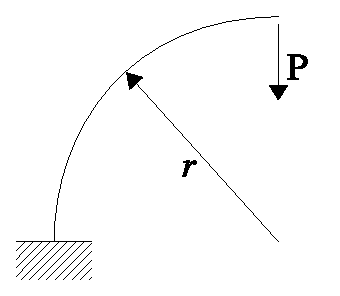
\includegraphics{curved_beam}
\centering
\caption{Schematic for the static deformation of a curved beam}
\label{fig:curved_beam}
\end{figure}
A schematic is shown in figure \ref{fig:curved_beam}.
This problem has a semi-analytic solution, given in Timoshenko's \emph{Strength of Materials, Vol I}.  
The displacement in the vertical direction (in the direction of $P$) is
\begin{equation} \delta_y = \frac{\pi}{4} \frac{P r^3}{EI} \label{eq:eq10000} \end{equation}
and the horizontal displacement (to the right) is
\begin{equation}  \delta_x = \frac{Pr^3}{2EI} \label{eq:eq10100} \end{equation}
Consider a beam with 
\[ I/b = 6.66667 \times 10^{-7} \]
\[ E = 2.1 \times 10^{11} \]
\[ r = 1 \]
loaded with a force
\[ P/b = 1 \]
The semi-analytical $y$ displacement from (\ref{eq:eq10000}) is
\[ \delta_y = 5.6099866 \times 10^{-6} \]
and the $x$ displacement from (\ref{eq:eq10100}) is
\[ \delta_x = 3.571428 \times 10^{-6} \]
Discretizing this beam with 30 elements and simulating, we get from the nonlinear finite element model
\[ \delta_y = 5.614 \times 10^{-6} \]
and
\[ \delta_x = 3.57533 \times 10^{-6} \]
which is in very good agreement with the solution from Timoshenko's book.

\item Turek \& Hron CSM Benchmark (1).

The paper by Turek and Hron \cite{TurekHron2006} also contains two static test cases.  
Both cases use a 0.35 m beam, which is 0.02 m thick, cantilevered on the left end and free on the right end.
Furthermore, in both cases the beams are loaded only with a gravitational body force, ${\bf g} = (0,-2) \ \mbox{m/s$^2$}$.

In the first case, the properties of the beam are
\[ \rho = 1000 \mbox{ kg/m$^3$} \]
\[ \nu = 0.4 \]
\[ E = 5.6 \times 10^6 \mbox{ kg/m s$^2$} \]
Now it appears that the benchmark case provided assumes that the structure is in a state of plane strain, whereas the beam model described herein assumes that the beam is in a state of plane stress. 
To get comparable results, then, we must adjust the elastic modulus slightly:
\[ \bar{E} = \frac{E}{1-\nu^2} = 6.666 \times 10^6 \mbox{ kg/m s$^2$} \]
For their simulation, Turek \& Hron obtain a tip displacement of 
\[ \delta_x = -0.4690 \times 10^{-3} \mbox{ m} \]
and 
\[ \delta_y = -16.97 \times 10^{-3} \mbox{ m} \]
For our model, we obtain
\[ \delta_x = -0.4669 \times 10^{-3} \mbox{ m} \]
and 
\[ \delta_y = -16.904 \times 10^{-3} \mbox{ m} \]
Our model yields the same result to two/three decimal places.
This is good agreement considering that we use a simplified beam model, whereas the reference solution uses solid elements.

\item Turek \& Hron CSM Benchmark (2).

The second benchmark is similar to the first, except that the elastic modulus is set to
\[ E = 1.4 \times 10^6 \mbox{ kg/m s$^2$} \]
We again have to adjust the elastic modulus slightly, yielding
\[ \bar{E} = 1.666 \times 10^6 \mbox{ kg/m s$^2$} \]
For their simulation, Turek \& Hron obtain a tip displacement of 
For our model, we obtain
\[ \delta_x = -7.187 \times 10^{-3} \mbox{ m} \]
and 
\[ \delta_y = -66.10 \times 10^{-3} \mbox{ m} \]
For our model, we obtain
\[ \delta_x = -7.165 \times 10^{-3} \mbox{ m} \]
and 
\[ \delta_y = -65.875 \times 10^{-3} \mbox{ m} \]
For this case, we see agreement to roughly two decimal places.

\end{enumerate}
\subsection{Dynamic test cases}
\begin{enumerate}
\item Turek \& Hron CSM Benchmark (3).

This is the same as the static benchmark \emph{Turek \& Hron CSM Benchmark (2)}, except that it is dynamic. 
The beam is started from a straight, undeformed configuration, with zero velocity, and then permitted to fall and oscillate under the influence of gravity.
They present an oscillatory response, with an \emph{x} displacement of the tip varying between
\[ \delta_x \in [0,-28.61] \times 10^{-3} \mbox{ m} \]
and a \emph{y} displacement varying between
\[ \delta_y \in [1.553,-128.8] \times 10^{-3} \mbox{ m} \]
and a period of
\[ T = 0.9095 \mbox{ s} \]
Performing the simulation in our code, we get the following plots for the tip displacement (c.f. the plots in the Turek \& Hron paper):
\begin{figure}[ht]
        \centering
        \subfigure[X displacement]{ %{0.4\textwidth}
                \centering
                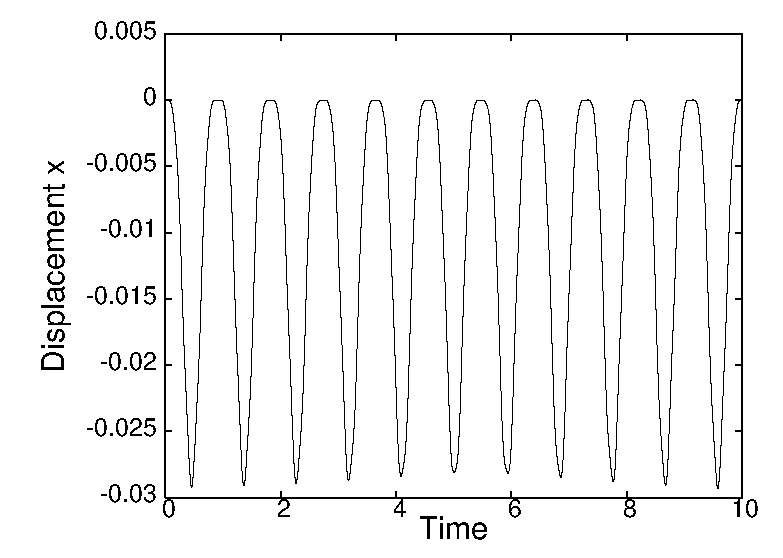
\includegraphics[width=0.4\textwidth]{displacement_x1}
                \label{fig:TurekHronDisplacementCSM3X1}
        }
        \subfigure[Y displacement]{%{0.4\textwidth}
                \centering
                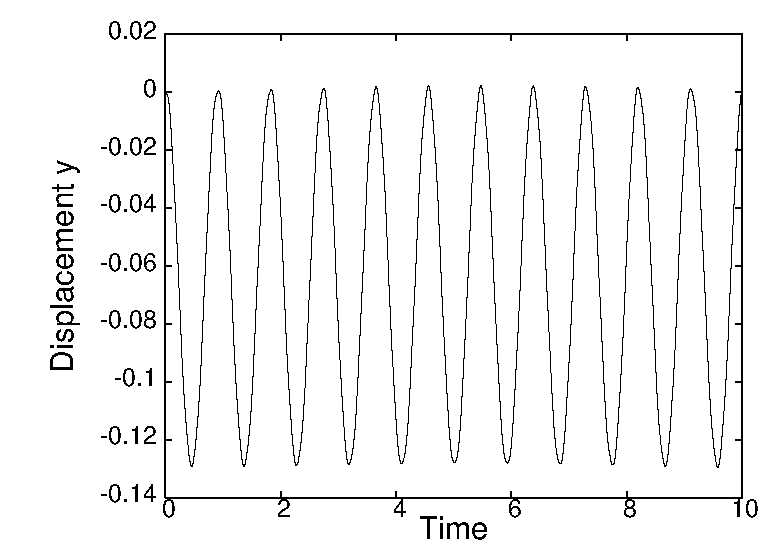
\includegraphics[width=0.4\textwidth]{displacement_y1}
                \label{fig:TurekHronDisplacementCSM3Y1}
        }
        \caption{Tip displacements for the Turek \& Hron CSM Benchmark (3)}
\end{figure}

\begin{figure}[ht]
        \centering
        \subfigure[X displacement]{ %{0.4\textwidth}
                \centering
                \includegraphics[width=0.4\textwidth]{displacement_x2}
                \label{fig:TurekHronDisplacementCSM3X2}
        }
        \subfigure[Y displacement]{%{0.4\textwidth}
                \centering
                \includegraphics[width=0.4\textwidth]{displacement_y2}
                \label{fig:TurekHronDisplacementCSM3Y2}
        }
        \caption{Tip displacements for the Turek \& Hron CSM Benchmark (3)}
\end{figure}
\end{enumerate}
Qualitatively, these plots demonstrate that our model is in good agreement with the model from Turek \& Hron.  
Quantitatively, our response is also oscillatory, with the $x$ displacement during the time $t\in[8,10]$ varying between
\[ \delta_x \in [0.005,-29.3] \times 10^{-3} \mbox{ m} \]
and a \emph{y} displacement varying between
\[ \delta_y \in [1.5726,-129.6] \times 10^{-3} \mbox{ m} \]
The measured period for the $x$ displacement (e.g., between the two extrema in the time period $t\in[8,10]$) is 0.90687 s, and for the $y$ displacement 0.91258 s. 
There is a slight discrepancy in the periods because our model seems to have a weak second mode (which can be seen in figure \ref{fig:TurekHronDisplacementCSM3X1}).
This mode does not seem present in the model of Turek \& Hron.
Despite this, both computed periods are very close to the reference value given by Turek \& Hron.

\subsection{FSI Coupling}
The overall coupling procedure is the same as in the linear beam case.  
Two elements are worthy of note however: (1) The construction of the boundary mesh, and (2) the integration of the fluid loads.
\subsubsection{Boundary mesh construction}
A naive approach to constructing the fluid boundary mesh (i.e., the wetted surface) would be to simply connect adjacent slave nodes with straight lines.
While appealing, this would result in a boundary mesh that is not smooth.
Instead, our construction will consist of two steps which will guarantee the smoothness of the resulting boundary mesh.
First, on each element $E$ with master nodes $i$ and $i+1$,  we construct a cubic Bezier curve connecting these two nodes, ${\bf B}(s)$.  
We then the boundary curve is defined to be
\begin{subequations}
\label{equations3}
\begin{align}
  \label{eq:eq11100a}
  \tilde{x} &= B_x(s) + \cos{(\theta(s))} d(s) - \delta_x(s)  \\
  \label{eq:eq11100b}
  \tilde{y} &= B_y(s) + \sin{(\theta(s))} d(s) - \delta_y(s) 
\end{align}
\end{subequations}
where $s \in [0,1]$.
The functions $d(s)$, $\delta_x(s)$, and $\delta_y(s)$ are defined using the initial boundary mesh from the mesh generator.
For any boundary point $p_i = (x_{i,0},y_{i,0})$, we determine at the beginning of the simulation (in the undeformed configuration) which master element $E$ the boundary point is closest to (note that the master element $E$ is geometrically a line segment).
This point $p$ is then projected onto the element $E$, yielding a distance, $d_i$, and a natural coordinate, $\xi_i$, which describes where the projection of $p_i$ is within the element $E$.
There is a one-to-one correspondence between $s$ and $\xi$,
\[ s_i = \frac{1}{2}\xi_i + \frac{1}{2} \]
The function $d$ then satisfies
\[ d(s_i) = d_i \]
The functions $\delta_x(s)$, and $\delta_y(s)$ are defined so that at $t=0$, $\tilde{x}_i = x_{i,0}$ and  $\tilde{y}_i = y_{i,0}$.
It remains now to construct the Bezier curve  ${\bf B}(s)$. 
A cubic Bezier curve takes the form
\begin{equation} \mathbf{B}(s) = (1-s)^3\mathbf{P}_0 + 3(1-s)^2s\mathbf{P}_1 + 3(1-s)s^2\mathbf{P}_2+s^3\mathbf{P}_3 \label{eq:eq10300} \end{equation}
This curve goes through $\mathbf{P}_0$ at $s=0$, and $\mathbf{P}_1$ at $t=1$. 
In addition, it is tangent to the line segment $\overline{\mathbf{P}_0\mathbf{P}_1}$ at $s=0$, and tangent to the line segment $\overline{\mathbf{P}_2\mathbf{P}_3}$ at $s=1$.
To guarantee smoothness, we will require that the curve pass through the two master nodes $i$ and $i+1$, and that the curve be perpendicular to the directors at these nodes.
To construct this curve between master nodes defined by $(x_i, y_i)$ and $(x_{i+1}, y_{i+1})$, we first set 
\[ \mathbf{P}_0 = (x_i, y_i) \mbox{ , } \mathbf{P}_3 = (x_{i+1}, y_{i+1}) \]
We wish $\mathbf{B}(s)$ to be perpendicular to the director $\mathbf{p}_i$ at $\mathbf{P}_0$, and perpendicular to the director $\mathbf{p}_{i+1}$ at $\mathbf{P}_3$.
This requires that 
\begin{subequations}
\label{equations4}
\begin{align}
 \label{eq:eq10400a}
 \mathbf{P}_1 &= \mathbf{P}_0 + \zeta \mathbf{p}_i^{\bot} \\
 \label{eq:eq10400b}
 \mathbf{P}_2 &= \mathbf{P}_3 - \zeta \mathbf{p}_{i+1}^{\bot} \\
\end{align}
\end{subequations}
where $\mathbf{p}_i^{\bot}$ is a vector perpendicular to $\mathbf{p}_i$ pointing in the direction from $i$ to $i+1$.  
The scale factor $\zeta$ is somewhat arbitrary.  
I choose
\begin{equation}  \zeta = \frac{1}{3}\| \mathbf{P}_3 - \mathbf{P}_0 \| \label{eq:eq10500} \end{equation}
though I imagine many other choices are possible.
One advantage of using this sort of curve for the boundary mesh is that in addition to being easy to construct, it is also simple to obtain the acceleration of points on the boundary (which is necessary to perform the FSI coupling).
From (\ref{eq:eq11100a}), (\ref{eq:eq11100b}), we have
\begin{equation} \ddot{\bf x} = \frac{\partial^2 \mathbf{B}(s)}{\partial t^2} + d(s)\left( -\omega^2\begin{bmatrix} \cos \theta \\ \sin \theta \end{bmatrix} + \ddot{\omega} \begin{bmatrix} -\sin \theta \\ \cos \theta \end{bmatrix} \right) \label{eq:eq10550} \end{equation}
The partial of the Bezier spline can be computed:
\begin{equation}  \frac{\partial^2 \mathbf{B}(s)}{\partial t^2} = (1-s)^3\frac{\partial^2 \mathbf{P}_0}{\partial t^2} + 3(1-s)^2s\frac{\partial^2 \mathbf{P}_1}{\partial t^2} + 3(1-s)s^2\frac{\partial^2 \mathbf{P}_2}{\partial t^2}+s^3\frac{\partial^2 \mathbf{P}_3}{\partial t^2} \label{eq:eq10600} \end{equation}
Now
\[ \mathbf{P}_0 = \mathbf{x}_i + \frac{1}{2}h_0 \mathbf{p}_i \]
so
\begin{equation}  \frac{\partial^2 \mathbf{P}_0}{\partial t^2} = \mathbf{a}_i + \frac{1}{2}h_0 \left(-\omega_i^2 \mathbf{p}_i -\alpha_i \mathbf{p}_i^{\bot}\right) \label{eq:eq10700} \end{equation}
and 
\begin{equation}  \frac{\partial^2 \mathbf{P}_3}{\partial t^2} = \mathbf{a}_{i+1} + \frac{1}{2}h_0 \left(-\omega_{i+1}^2 \mathbf{p}_{i+1} -\alpha_{i+1} \mathbf{p}_{i+1}^{\bot}\right)  \label{eq:eq10800} \end{equation}
Now I approximate
\begin{equation} \frac{\partial^2 \mathbf{P}_1}{\partial t^2} = \frac{\partial^2 \mathbf{P}_0}{\partial t^2} + \zeta \left( -\omega_i^2\mathbf{p}_i^{\bot}+\alpha_i \mathbf{p}_i \right) \label{eq:eq10900} \end{equation}
and
\begin{equation} \frac{\partial^2 \mathbf{P}_2}{\partial t^2} = \frac{\partial^2 \mathbf{P}_3}{\partial t^2} - \zeta \left( -\omega_{i+1}^2\mathbf{p}_{i+1}^{\bot}+\alpha_{i+1} \mathbf{p}_{i+1} \right) \label{eq:eq11000} \end{equation}
Note that this ignores the dependence of $\zeta$ on $t$, but I think this effect is minimal at best.  
If desired this can be rectified either by using a formula for $\zeta$ that does not depend on $t$, or by including the dependence of $\zeta$ on $t$ in the derivative formulas.
I see no evidence that this is necessary, however.

\subsubsection{Load computation}
The computation of the external load is actually simpler than it is for the linear beam.
The external load is first computed at the slave nodes.
On the top surface of the beam (which corresponds to $\eta = 1$) we have
\begin{equation} {\bf f}_{e, \mbox{slave}} = \int N(\xi, 1) \mathbf{t} \left| \frac{\partial s}{\partial \xi}\right| \ d\xi \label{eq:eq11200} \end{equation}
where $\mathbf{t}$ is the traction vector.
At the moment, I assume 
\[ \mathbf{t} = p(\xi) \mathbf{n} \]
thereby neglecting viscous forces.  
Further, I assume $p(\xi)$ to be a piecewise linear function, in particular linear on each element of the boundary mesh (not each element of the structural mesh).
I also take $\mathbf{n}$ to be constant on each boundary mesh element.
As before, I assume other (or better) approximations are possible for $p(\xi)$ and $\mathbf{n}$; however, I have no evidence that these are necessary.
Clearly, though, neglecting the viscous forces is not a good approximation.  
For studying FSI coupling in viscous incompressible flows, however, in which the pressure forces are dominant (and the dominant causes of instability), it is reasonable.  
This is not to say that adding the viscous forces is difficult; rather it is quite trivial.

The external forces at the master nodes can then be obtained utilizing a similar transformation as that used for the internal forces.
\[ {\bf f}_{e,\mbox{master,I}} = {\bf T}_I^T \left[ \begin{array}{c} f_{e, \mbox{slave,I}-}^x \\  f_{e, \mbox{slave,I}-}^y \\ f_{e, \mbox{slave,I}+}^x \\  f_{e, \mbox{slave,I}+}^y \end{array} \right]  \]

\subsection{FSI test cases}
\begin{enumerate}
\item Turek \& Hron FSI Benchmark (1).

This test case involves a thin, flexible beam, mounted on the back of a cylinder (e.g., like a streamer).
The beam has the same geometry as in the dynamic test case \emph{Turek \& Hron CSM Benchmark (1)}: 0.35 m long, 0.02 m thick.  
The density of the beam is $\rho_s = 10^4 \mbox{ kg/m$^3$}$, with Poisson's ratio $\nu = 0.4$ and elastic modulus $E = 1.4 \times 10^6 \mbox{ Pa}$.  
Note that as before we must adjust the elastic modulus slightly to account for the fact that our beam model assumes plane stress, whereas the Turek \& Hron results are presented for a structure in plane strain (or they appear to be).

A cartoon of the problem geometry is shown in figure \ref{fig:TurekHronGeometryFSI2}.
\begin{figure}[ht]
        \centering
        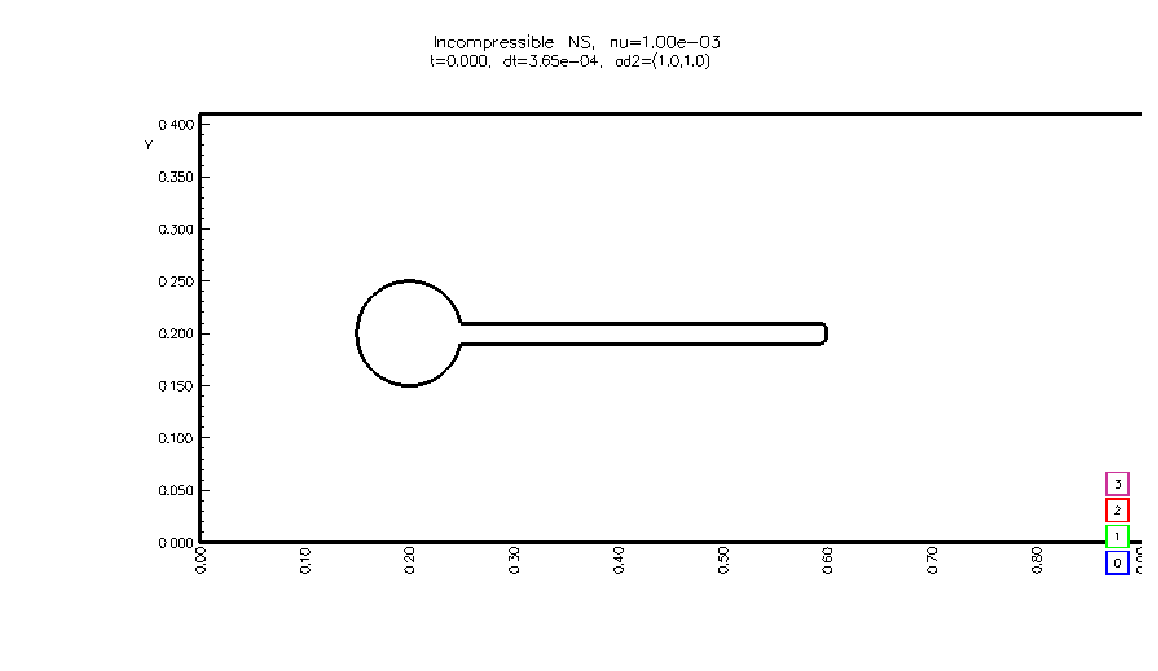
\includegraphics[width=\textwidth]{elastic_flag_geom} 
        \caption{Geometry of the Turek \& Hron FSI Benchmark (1)}
        \label{fig:TurekHronGeometryFSI2}.
\end{figure}
For a full desciption of the problem geometry, the reader is referred to the original paper. 
The inflow flow profile (at the left) is set to be parabolic and time dependent, with flow in the \emph{x} direction, with velocity:
\begin{equation}  u(t,0,y) = 1.5\bar{U}\frac{y(H-y)}{(H/2)^2}\times \left\{ \begin{array}{ll} \frac{1-\cos{\frac{\pi}{2}t}}{2} & t < 2 \\ 1 & \mbox{otherwise} \end{array} \right. \label{eq:eq11300} \end{equation}
where $H = 0.41 \mbox{ m}$ is the height of the domain and $\bar{U}$ is the average inflow velocity.  
For this case, $\bar{U}$ is set to $1 \mbox{ m/s}$. 
Further, the fluid uses has a density $\rho^f = 10^3 \mbox { kg/m$^3$}$ and kinematic viscosity $\nu^f = 10^{-3} \mbox { m$^2$/s}$.
After a period of time, the beam enters into a steady (or nearly steady) oscillation.  
The oscillatory response presented by Turek \& Hron is characterized by an \emph{x} displacement of the tip varying between
\[ \delta_x \in [-2.14,27.02] \times 10^{-3} \mbox{ m} \]
with a period of
\[ T_x = 0.26 \mbox{ s} \]
and a \emph{y} displacement varying between
\[ \delta_y \in [81.83,-79.37] \times 10^{-3} \mbox{ m} \]
with a period of
\[ T_y = 0.50 \mbox{ s} \]
Performing the simulation in our code, we get the following plots for the tip displacement (c.f. the plots in the Turek \& Hron paper):
\begin{figure}[ht]
        \centering
        \subfigure[X displacement]{ %{0.4\textwidth}
                \centering
                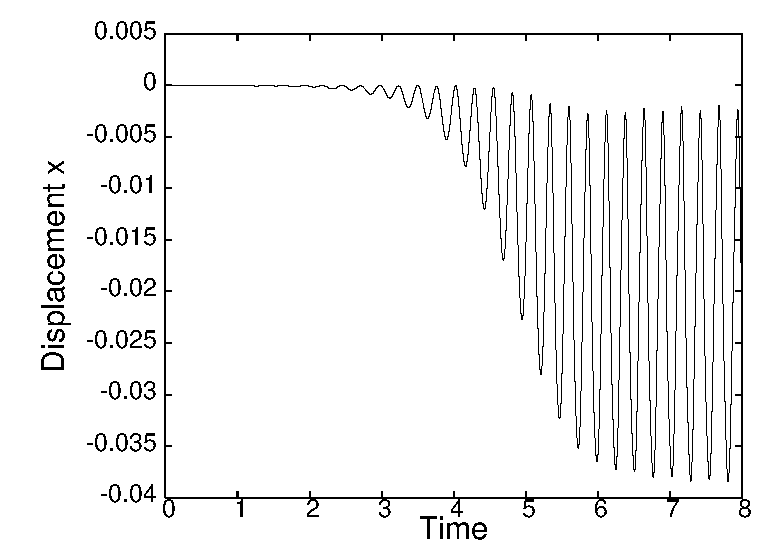
\includegraphics[width=0.4\textwidth]{displacement_fsi2_x1}
                \label{fig:TurekHronDisplacementFSI2X1}
        }
        \subfigure[Y displacement]{%{0.4\textwidth}
                \centering
                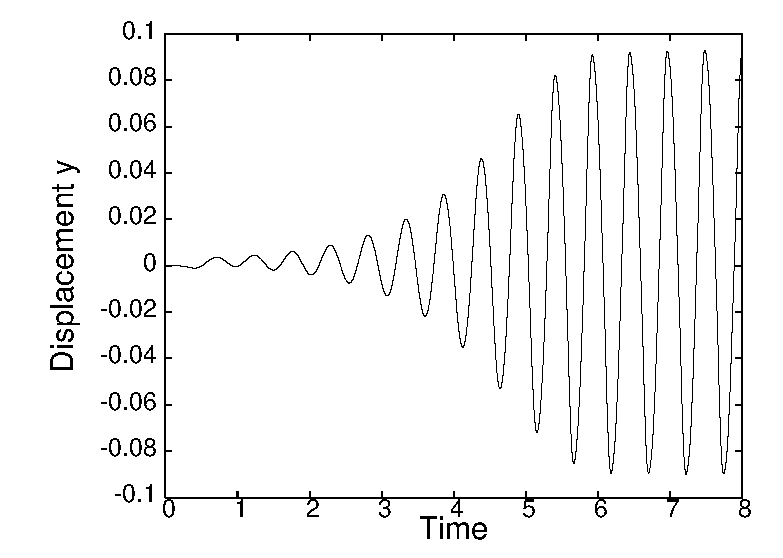
\includegraphics[width=0.4\textwidth]{displacement_fsi2_y1}
                \label{fig:TurekHronDisplacementFSI2Y1}
        }
        \caption{Tip displacements for the Turek \& Hron FSI Benchmark (1)}
\end{figure}

\begin{figure}[ht]
        \centering
        \subfigure[X displacement]{ %{0.4\textwidth}
                \centering
                \includegraphics[width=0.4\textwidth]{displacement_fsi2_x2}
                \label{fig:TurekHronDisplacementFSI2X2}
        }
        \subfigure[Y displacement]{%{0.4\textwidth}
                \centering
                \includegraphics[width=0.4\textwidth]{displacement_fsi2_y2}
                \label{fig:TurekHronDisplacementFSI2Y2}
        }
        \caption{Tip displacements for the Turek \& Hron FSI Benchmark (1)}
\end{figure}
From these plots, the \emph{x} displacement in the (nearly-) steady state oscillation varies between
\[ \delta_x \in [-1.97,-38.5] \times 10^{-3} \mbox{ m} \]
with a period of
\[ T_x = 0.26 \mbox { s} \]
and a \emph{y} displacement varying between
\[ \delta_y \in [-89.9,92.9] \times 10^{-3} \mbox{ m} \]
and a period of
\[ T_y = 0.52 \mbox{ s} \]
The measured periods are nearly identical.  
However, the computed oscillations of the beam are about 10\% larger (based on the \emph{y} displacement) than those from the Turek \& Hron reference.  
This is not surprising, though, because in our model we have not added the viscous forces to the load computation.  
It is actually expected, therefore, that there is some discrepancy between the results from our model and the Turek \& Hron reference.

\item Turek \& Hron FSI Benchmark (2).

This case is very similar to the previous case, \emph{Turek \& Hron FSI Benchmark (1)}.
Furthermore, the density of the beam is $\rho_s = 10^3 \mbox{ kg/m$^3$}$, with Poisson's ratio $\nu = 0.4$ and elastic modulus $E = 5.6 \times 10^6 \mbox{ Pa}$.  
Note that as before we must adjust the elastic modulus slightly to account for the fact that our beam model assumes plane stress, whereas the Turek \& Hron results are presented for a structure in plane strain (or it appears to be).
The problem geometry and fluid properties are the same as before.  
The initial conditions are also the same, except that the mean inflow velocity is increased to $\bar{U} = 2 \mbox{ m/s}$.
After a period of time, the beam enters into a steady (or nearly steady) oscillation.  
Their oscillatory response is characterized by an \emph{x} displacement of the tip varying between
\[ \delta_x \in [-0.16,-5.22] \times 10^{-3} \mbox{ m} \]
with a period of
\[ T_x = 0.0917 \mbox{ s} \]
and a \emph{y} displacement varying between
\[ \delta_y \in [-32.90,35.86] \times 10^{-3} \mbox{ m} \]
and a period of
\[ T_y = 0.19 \mbox{ s} \]
Performing the simulation in our code, we get the following plots for the tip displacement (c.f. the plots in the Turek \& Hron paper):
\begin{figure}[ht]
        \centering
        \subfigure[X displacement]{ %{0.4\textwidth}
                \centering
                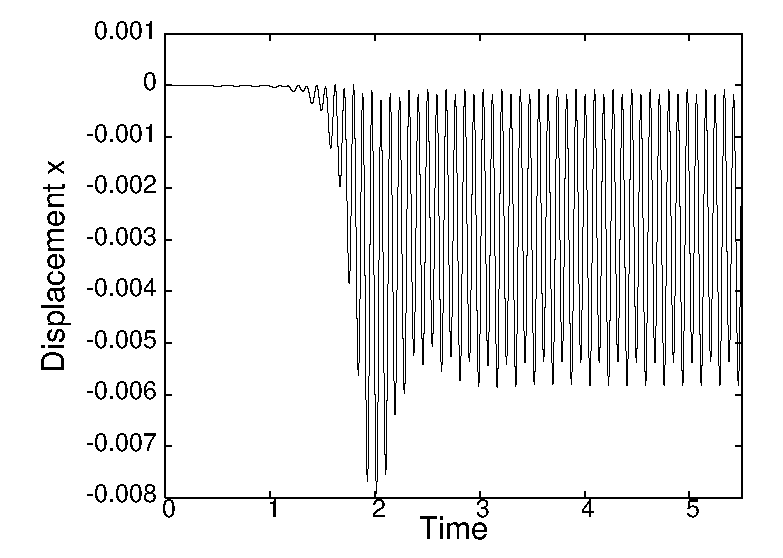
\includegraphics[width=0.4\textwidth]{displacement_fsi3_x1}
                \label{fig:TurekHronDisplacementFSI3X1}
        }
        \subfigure[Y displacement]{%{0.4\textwidth}
                \centering
                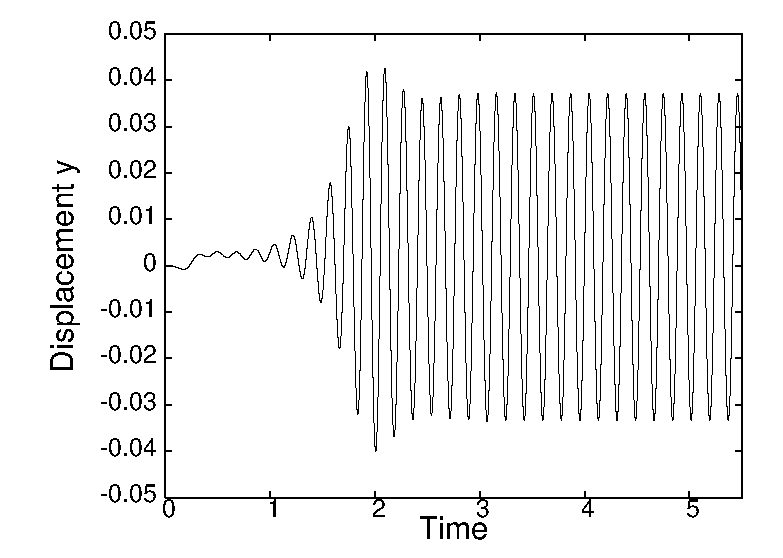
\includegraphics[width=0.4\textwidth]{displacement_fsi3_y1}
                \label{fig:TurekHronDisplacementFSI3Y1}
        }
        \caption{Tip displacements for the Turek \& Hron FSI Benchmark (2)}
\end{figure}

\begin{figure}[ht]
        \centering
        \subfigure[X displacement]{ %{0.4\textwidth}
                \centering
                \includegraphics[width=0.4\textwidth]{displacement_fsi3_x2}
                \label{fig:TurekHronDisplacementFSI3X2}
        }
        \subfigure[Y displacement]{%{0.4\textwidth}
                \centering
                \includegraphics[width=0.4\textwidth]{displacement_fsi3_y2}
                \label{fig:TurekHronDisplacementFSI3Y2}
        }
        \caption{Tip displacements for the Turek \& Hron FSI Benchmark (2)}
\end{figure}
From these plots, the \emph{x} displacement in the (nearly-) steady state oscillation varies between
\[ \delta_x \in [-0.08,-5.82] \times 10^{-3} \mbox{ m} \]
with a period of
\[ T_x = 0.089 \mbox { s} \]
and a \emph{y} displacement varying between
\[ \delta_y \in [-33.31 ,37.11] \times 10^{-3} \mbox{ m} \]
and a period of
\[ T_y = 0.18 \mbox{ s} \]
We get a relatively good agreement between our results and the Turek \& Hron reference result.  
Our periods are slightly shorter, and the peak $x$ displacement is slightly larger than that of  Turek \& Hron.  
The plot in figure \ref{fig:TurekHronDisplacementFSI3X2} also shows a noticeable second mode, in addition to the one used to compute the period of oscillation.  
This mode is also evident when examining the plots from the  Turek \& Hron paper, however its amplitude is somewhat less pronounced.
The $y$ displacements agree quite well.  
\end{enumerate}

\section{Future work}
The nonlinear beam model described in the previous section can easily be extended to handle three dimensional beams (also called risers).
The same general assumptions made in the two dimensional beam model can be made in the three dimensional model.
We still define the beam using a set of master nodes down the center of the beam.
In three dimensions, instead of having quads as slave elements we will have hexes -- so that every master node has four slave nodes associated with it rather than two.
Further, whereas in two dimensions the slave nodes were defined using a single director ${\bf p}_i$, (equations (\ref{eq:eq6800a}, \ref{eq:eq6800b})), now there are two directors at each slave node, ${\bf p}_i^1$ and ${\bf p}_i^2$.
The slave node positions are then 
\begin{equation} {\bf x}_i^{\mbox{slave}} = {\bf x}_i \pm \frac{1}{2}h_i^1  {\bf p}_i^1 \pm  \frac{1}{2}h_i^2  {\bf p}_i^2 \label{eq:eq11400} \end{equation}
These directors can be defined by creating a local coordinate system at ${\bf x}_i$ whose rotation is specified by the quaternion ${\bf q}_i$.
The internal force calculation (equation (\ref{eq:eq7300}) in 2D) is very similar, except that we must now enforce both $\mathbf{\sigma}_{\hat{y}\hat{y}} = 0$ and $\mathbf{\sigma}_{\hat{z}\hat{z}} = 0$.  
The plane stress assumption, though, no longer applies.  
In order to satisfy the condition on the normal stresses, we must modify the strain components (or strain deformation components, depending on the material model).
In the SVK material model, this would correspond to modifying $E_{\hat{y}\hat{y}},\ E_{\hat{z}\hat{z}}$ to maintain the zero normal stress condition in the beam.
The existence of complex cross sections (those that are not a box!) is one complication that does not exist in the two dimensional case.
The integral over the section necessary to compute the internal force must be split up into pieces.  
My suggestion, similar to one from the LS-DYNA documentation \cite{Hallquist1993}, is to supply a mesh of the cross section in simple shapes, either in triangles or quads.  
Having such a mesh makes performing the integrals in the internal force formulae possible to do with straightforward Gaussian quadrature on each shape.
The matrix transformation ${\bf T}$ as well as the stiffness matrices will be slightly different, but maintain the same form.
Caution must be exercised when integrating the rotational degrees of freedom, due to the nonlinear relationship between the angular velocity and quaternion temporal derivatives; however, this relationship is well documented in the rigid body dynamics literature.
A beam implemented in this way would allow all of the major deformational modes possible for bars: extension, bending about any axis, and torsion.

The load computation is a trivial extension of equation (\ref{eq:eq11200}).  
The update of the boundary mesh requires some elucidation.  
We start with the three dimensional extensions of equations (\ref{eq:eq11100a}) and (\ref{eq:eq11100b}):
\begin{equation} \tilde{\bf x} = {\bf B}(s) + {\bf p}^1(s) d^1(s) + {\bf p}^2(s) d^2(s) - \mathbf{\delta}(s) \label{eq:eq11500} \end{equation}
where ${\bf p}^1(s)$ and ${\bf p}^2(s)$  are the interpolated directors at $s$ (where $s$ is defined analogously to the two dimensional case), and $\mathbf{\delta}(s)$ is similary defined so that $\tilde{\bf x} = {\bf x}_0$ at $t=0$.
The Bezier curve ${\bf B}(s)$ is now a three dimensional curve, and is constructed so as to pass through the appropriate master nodes ${\bf x}_i$ and ${\bf x}_{i+1}$, and to be perpendicular to both directors at these nodes. 
\appendix
\section{Nonlinear beam model format}
This appendix documents the format of the beam file used for the nonlinear beam.
The format is as follows: \\ \\
\texttt{ [\# master nodes] [\# master elements]} \\
\texttt{ [density] [nu] [Em] [omega\_structure] [isSteady]} \\
\texttt{ [bcLeft] [bcRight] } \\
\texttt{ [pressureNorm] [useExactSolution] [rayleighAlpha] [rayleighBeta] } \\
\texttt{ [X\_1] [Y\_1] [Z\_1] [$\Theta$\_1] [h\_1]} \\
\texttt{ [X\_2] [Y\_2] [Z\_2] [$\Theta$\_2] [h\_2]} \\
\texttt{ [X\_3] [Y\_3] [Z\_3] [$\Theta$\_3] [h\_3]} \\
\ldots \\
\texttt{ [X\_N] [Y\_N] [Z\_N] [$\Theta$\_N] [h\_N]} \\ \\
The parameters are  \\
\texttt{ [\# master nodes]}: Number of nodes placed along the center line of the beam \\
\texttt{ [\# master elements]}: Number of beam elements.  This should always be set to \texttt{ [\# master nodes]-1} \\
\texttt{ [density]}: Density of the beam \\
\texttt{ [nu]}: Poisson's ratio for the beam \\
\texttt{ [Em]}: Elastic modulus for the beam \\
\texttt{ [omega\_structure] }: Relaxation factor used when solving the nonlinear structural equations.  Should be set in the range $0 < \omega < 1$.  $1$ is typical, except when solving static equations, in which smaller factors may be necessary. \\
\texttt{ [isSteady] }: Set to 1 when solving static problems (for debugging), 0 otherwise (for FSI). \\
\texttt{ [bcLeft], [bcRight] }: Boundary condition on the left/right of the beam.  0 = cantilevered, 1 = pinned, and 2 = free. \\
\texttt{ [pressureNorm] }: Scale factor applied to the pressure obtained from the flow solver before computing the fluid load on the beam. \\
\texttt{ [useExactSolution] }:  Not used.  Set to zero. \\
\texttt{ [rayleighAlpha], [rayleighBeta]  }: Parameter $\alpha,\beta$ for damping.  $\alpha=\beta = 0$ corresponds to no damping. \\
\texttt{ [X\_i ], [Y\_i ],[Z\_i]  }: Undeformed position of master node $i$.  $Z_i$ should be set to zero. \\
\texttt{ [$\Theta$\_1] }: Initial, undeformed angle of the director with respect to the $x$ axis.  The director should generally be as perpendicular as possible to the neutral axis of the beam.
\texttt{ [h\_i] }: Thickness of the beam at node $i$.
The total number of lines specifying the nodes (i.e., $N$) must be the same as the number of master nodes specified, \texttt{ [\# master nodes]}.

\begin{thebibliography}{9}

\bibitem{Belytschko2000}
  Belytschko, T., Liu, W.K., Moran, B. 
  \emph{Nonlinear Finite Elements for Continua and Structures}.
  John Wiley \& Sons,
  2000.

\bibitem{Causin2004}
  Causin, P., Gerbeau, J-F., Nobile, F.
  \emph{Added-mass effect in the design of partitioned algorithms for fluid-structure problems}.
  INRIA report 5084,
  2004.

\bibitem{Giordano2005}
  Giordano, G., Jourdan, G., Burtschell, Y., Medale, M., Zeitoun, D.E., Houas, L.
  \emph{Shock wave impacts on deforming panel, an application of fluid-structure interaction}.
  Shocks Waves,
  2005.

\bibitem{Hallquist1993}
  Hallquist, J.O.
  \emph{LS-DYNA3D Theoretical Manual}.
  LSTC Report 1018 Rev. 2,
  1993.


\bibitem{TurekHron2006}
  Turek, S., Hron, J.
  \emph{Proposal for numerical benchmarking of fluid-structure interaction between an elastic object and laminar incompressible flow}.
  Springer,
  2006.


\end{thebibliography}

\end{document}
